\documentclass{these-seb}

\usepackage[utf8]{inputenc}
\usepackage[T1]{fontenc}
\usepackage{babel}

\usepackage{pifont}
% Les polices possibles (pour tout le document)
%\usepackage[bitstream-charter]{mathdesign}

%Font ps pour le pdf
\usepackage{pslatex}

%Hyperliens pour le pdf
\usepackage[pdfauthor   = {Sébastien\ Le\ Roux},
    pdftitle    = {atomes\ user\ manual},
    pdfsubject = {atomes\ user\ manual\ documentation},
    pdfkeywords = {atomes\ user\ manual\ guide\ help\ documentation},
    pdfcreator = {Latex+DviPDF},
    pdfproducer = {LaTeX+DviPDF},
    pdfstartview=FitV   % Ouverture avec ajustement de l'image
    dvips=true,         % Use hyperref with dvips
    colorlinks=true,    % Lien hypertext en couleur
    plainpages=false,   %
    pagebackref=true,   % Permet d'ajouter des liens retour dans la biblio ...
    backref=page,       % .. ces liens pointent vers les 'pages' des citations
    hyperindex=true,    % Ajoute des liens dans l'index
    linktocpage=true,   % Lien sur les numéros de page et non le text 
    breaklinks=true,    % Permet le retour à la ligne dans les liens trop longs
    urlcolor= blue,     % Couleur des liens externes
%    linkcolor= black,   % Couleur des liens internes
    bookmarks=true,     % Création des signets pour Acrobat
    bookmarksopen=false % Toute l'arborescence est dépliée à l'ouverture
]{hyperref}
%\usepackage[pageref]{backref}

%Insertion d'images
\usepackage{graphicx}
\DeclareGraphicsExtensions{.eps}

%Dessins latex
% Brouillon ? = afficher les images "false" ou seulement les cadres "true"
% effet sur tout le document
\newcommand{\ddst}{false}
%\usepackage{picins}

\usepackage{color}

% Mode verbatim avancé
\usepackage{alltt}

% Système de liste/énumération
\usepackage{pifont}
\usepackage{enumerate}

% Ecriture des mathématiques
\usepackage{amsmath}
\usepackage{amssymb}
\usepackage{amscd}
\usepackage{theorem}

\usepackage{pxfonts}

% tableaux
\usepackage{hhline}
%\usepackage{array}
\usepackage{multirow}
\usepackage{tabls}

%% Mise en page
\voffset         0.0cm
\hoffset         0.0cm
\textheight     24.0cm
\textwidth      16.0cm
\topmargin      -0.5cm
\oddsidemargin   0.0cm
\evensidemargin  0.0cm

% pages en landscape dans document portrait
\usepackage{lscape}

% Aspect de pages
\usepackage{setspace}
%\onehalfspacing
%\doublespacing
%\setstretch{3}

%\usepackage{fancyhdr,fancybox}
%\fancyhead{}
%\fancyhead[RO]{\scriptsize{\slshape\rightmark}}
%\fancyhead[LO]{\scriptsize{\thepage}}
%\fancyhead[RE]{\scriptsize{\thepage}}
%\fancyhead[LE]{\scriptsize{\slshape\leftmark}}
%\pagestyle{fancy}

% Numérotation pour les sous-sous-sections
\setcounter{secnumdepth}{3}
% Table des matières/figures/tables par chapitre
%\usepackage{minitoc}
% Pour placer des notes de bas de pages dans les titres
%\usepackage[stable]{footmisc}

%Définitions de théorèmes
\theoremstyle{plain}
\theoremheaderfont{\scshape}
\theorembodyfont{\normalfont\itshape}
\newtheorem{HK}{Théorème}

% Créer un environnement résumé
\def\abstract{
   \begin{center}
   \begin{minipage}{12cm}
   \begin{center}{\bf Résumé}\end{center}\par\small}
\def\endabstract{\par\end{minipage}\end{center}\vspace{1cm}}

% Bilblio:
\input{bibsymb}
%\usepackage{chapterbib}

%\usepackage[square,comma,sort&compress]{natbib}
%\usepackage{hypernat}

% Algo XML
\usepackage{listings}

% Texte souligné
\usepackage[normalem]{ulem}

% Mise en forme des légendes
\usepackage[hang]{caption2}
%\usepackage[hang]{caption}
\renewcommand{\captionfont}{\it}
\renewcommand{\captionlabelfont}{\bf}
\renewcommand{\captionlabeldelim}{$\quad$}

%\usepackage[format=plain,labelfont=bf,up,textfont=it,up]{caption}
\newcommand{\red}[1]{\textcolor{red}{#1}}
\newcommand{\blue}[1]{\textcolor{blue}{#1}}
\newcommand{\green}[1]{\textcolor{green}{#1}}
\newcommand{\violet}[1]{\textcolor{violet}{#1}}
\newcommand{\pink}[1]{\textcolor{pink}{#1}}
\newcommand{\aob}[1]{"{\texttt{#1}}"}

\definecolor{lg}{rgb}{0.95,0.95,0.95}

\newcounter{htmlkey}
\setcounter{htmlkey}{2}
\usepackage{keystroke}
\newcommand{\sclxml}{\input{sclxml}}
\newcommand{\sglxml}{\input{sglxml}}

\newcommand{\mbf}[1]{<#1>}
\newcommand{\key}[1]{\red{#1}}

\newcommand{\isaacs}{I.S.A.A.C.S.}
\newcommand{\ISAACS}{Interactive Structure Analysis of Amorphous and Crystalline Systems}
\newcommand{\atomes}{{\em{\bf{atomes}}}}
\newcommand{\activp}{{\em{\bf{active}}}}
\newcommand{\rpc}{$R_C(n)$}
\newcommand{\rpn}{$R_N(n)$}
\newcommand{\pnr}{$P_N(n)$}
\newcommand{\pnrmin}{$P_{N_{\text{min}}}(n)$}
\newcommand{\pnrmax}{$P_{N_{\text{max}}}(n)$}
\newcommand{\pmin}{$P_{\text{min}}(n)$}
\newcommand{\pmax}{$P_{\text{max}}(n)$}
\newcommand{\smin}{$s_{min}$}
\newcommand{\smax}{$s_{max}$}

\newcommand{\ges}{GeS$_2$}
\newcommand{\sio}{SiO$_2$}
\newcommand{\nn}{rings with $n$ nodes}
\newcommand{\con}{connectivity}
\newcommand{\conp}{connectivity profile}
\newcommand{\rstat}{ring statistics}

\newcommand{\dlpoly}{\href{https://www.scd.stfc.ac.uk/Pages/DL\_POLY.aspx}{DL-POLY}}
\newcommand{\lammps}{\href{https://lammps.sandia.gov/}{LAMMPS}}
\newcommand{\cpmd}{\href{http://www.cpmd.org}{CPMD}}
\newcommand{\cptk}{\href{http://cp2k.berlios.de}{CP2K}}

\newcommand{\atomesweb}{https://atomes.ipcms.fr}

\renewcommand{\figurename}{Figure}
\renewcommand{\tablename}{Table}
\newcommand{\laf}{\\}
\newcommand{\image}[2]{\includegraphics*[width=#1cm, keepaspectratio=true, draft=\ddst]{#2}}

\newcommand{\myfigure}[5]{\begin{figure}[!#1]{\hypertarget{#2}{\begin{center}{#3\caption[#4]{#5}\label{#2}}\end{center}}}\end{figure}}
\newcommand{\mytable}[5]{\begin{table}[!#1]{\begin{center}{#3\caption[#4]{#5}\label{#2}}\end{center}}\end{table}}

\newsavebox{\cobox}
\def\script{
  \noindent \laf \laf
  \begin{lrbox}
  \cobox
  \begin{minipage}[l]{16cm}
  \begin{alltt}}
\def\endscript{
  \end{alltt}
  \end{minipage}
  \end{lrbox}
  \colorbox{lg}{\usebox{\cobox}}
  \vspace{0.125cm}\par\noindent}

\def\scri#1{
  \noindent \laf \laf
  \begin{lrbox}
  \cobox
  \begin{minipage}[l]{#1cm}
  \begin{alltt}}
\def\endscri{
  \end{alltt}
  \end{minipage}
  \end{lrbox}
  \colorbox{lg}{\usebox{\cobox}}
  \vspace{0.25cm}\par\noindent}

\input{fig-data}
\input{tab-data}
\newcommand{\kbdmain}{
\begin{minipage}{8cm}
\begin{itemize}
\item Workspace: 
\item[] \Ctrl + \keystroke{w} : open workspace
\item[] \Ctrl + \keystroke{s} : save workspace as
\item[] \Ctrl + \keystroke{c} : close workspace \\
\item Project:
\item[] \Ctrl + \keystroke{n} : create new project
\item[] \Ctrl + \keystroke{o} : open project
\end{itemize}
\end{minipage}
\begin{minipage}{8cm}
\begin{itemize}
\item Misc:
\item[] \Ctrl + \keystroke{t} : show curve toolboxes
\item[] \Ctrl + \keystroke{p} : open periodic table
\item[] \Ctrl + \keystroke{a} : show about dialog
\item[] \Ctrl + \keystroke{q} : quit \\
\item On any file dialog:
\item[] \Ctrl + \keystroke{l} : open command line
\end{itemize}
\end{minipage}}

\newcommand{\kbdcurve}{
\begin{itemize}
\item Combined keys shortcuts:
\item[] \Ctrl + \keystroke{a} : Autoscale
\item[] \Ctrl + \keystroke{c} : Close curve window 
\item[] \Ctrl + \keystroke{e} : Open the data plot editing tool box [Fig.~\ref{edittool}]
\item[] \Ctrl + \keystroke{i} : Export image
\item[] \Ctrl + \keystroke{s} : Save / export data
\end{itemize}
}

\newcommand{\kbdviz}{
\begin{itemize}
\item Single key shortcuts:
\begin{itemize}
\item Colors:
\item[] \keystroke{a} : change atom(s) colormap
\item[] \keystroke{p} : change polyhedra(ons) colormap \\
\item Styles: 
\item[] \keystroke{b} : change default style to \aob{Ball and stick}  
\item[] \keystroke{c} : change default style to \aob{Cylinders}
\item[] \keystroke{d} : change default style to \aob{Dots} 
\item[] \keystroke{s} : change default style to \aob{Spheres} 
\item[] \keystroke{o} : change default style to \aob{Covalent radius}
\item[] \keystroke{i} : change default style to \aob{Ionic radius}
\item[] \keystroke{v} : change default style to \aob{van Der Waals radius}
\item[] \keystroke{r} : change default style to \aob{In cristal radius}
\item[] \keystroke{w} : change default style to \aob{Wireframe} \\
\item Measures: 
\item[] \keystroke{m} : show all measures for the selection, if pressed:
\begin{itemize}
\item once: display inter-atomic distance(s)
\item twice: display inter-atomic angles
\item a third time: hide measures \\
\end{itemize}
\item Model rotation:
\item[] \RArrow\ : rotate right
\item[] \LArrow\ : rotate left
\item[] \UArrow\ : rotate up
\item[] \DArrow\ : rotate down \\
\end{itemize}
\item Misc:
\item[] \Esc\ : exit fullscreen mode
\item[] \Spacebar\ : pause / restart spinning
%\item[] \Del : Delete all selected atom(s)
\newpage
\item Combined keys shortcuts:
\begin{itemize}
\item Mouse mode:
\item[] \Alt + \keystroke{a} : enter mouse \aob{Analysis} mode
\item[] \Alt + \keystroke{e} : enter mouse \aob{Edition} mode \\
\item Selection:
\item[] \Ctrl + \keystroke{a} : select / unselect all atoms
\item[] \Ctrl + \keystroke{c} : copy all selected atom(s)
%\item[] \Ctrl + \keystroke{v} : paste copied selection (if the model is not a MD trajectory)
%\item[] \Ctrl + \keystroke{x} : copy, then delete selection
%\item[] \Ctrl + \keystroke{n} : create new (empty project) \\
\item Mouse selection mode:
\item[] \Shift + \keystroke{a} : atom selection mode
\item[] \Shift + \keystroke{c} : coordination sphere selection mode
\item[] \Shift + \keystroke{f} : fragment selection mode
\item[] \Shift + \keystroke{m} : molecule selection mode \\	
\item Camera motion:
\item[] \Ctrl + \RArrow\ : move camera right
\item[] \Ctrl + \LArrow\ : move camera left
\item[] \Ctrl + \UArrow\ : move camera up
\item[] \Ctrl + \DArrow\ : move camera down
\item[] \Shift + \UArrow\ : zoom out
\item[] \Shift + \DArrow\ : zoom in \\
\item Spinning: 
\item[] \Ctrl + \Shift + \RArrow\ : spin right / increase speed right or reduce speed left
\item[] \Ctrl + \Shift + \RArrow\ : spin left / increase speed left or reduce speed right
\item[] \Ctrl + \Shift + \UArrow\ : spin up / increase speed up or reduce speed down
\item[] \Ctrl + \Shift + \DArrow\ : spin down / increase speed down or reduce speed up
\item[] \Ctrl + \keystroke{s} : stop spinning \\
\item Misc:
\item[] \Ctrl + \keystroke{l} : label / unlabel all atoms 
\item[] \Ctrl + \keystroke{e} : open the \aob{Environments configuration} window [Sec.~\ref{ecw}]
\item[] \Ctrl + \keystroke{m} : open the \aob{Measures} dialog [Sec.~\ref{mdw}]
\item[] \Ctrl + \keystroke{r} : open the \aob{Recorder} dialog [Sec.~\ref{rdw}]
\item[] \Ctrl + \keystroke{f} : enter / exit fullscreen mode 
\end{itemize}
\end{itemize}}

\newcommand{\kbdedit}{
\begin{itemize}
\item Single key shortcuts:
\begin{itemize}
\item Colors:
\item[] \keystroke{a} : change atom(s) colormap
\item[] \keystroke{p} : change polyhedra(ons) colormap \\
\item Styles: 
\item[] \keystroke{b} : change default style to \aob{Ball and stick}
\item[] \keystroke{c} : change default style to \aob{Cylinders}
\item[] \keystroke{d} : change default style to \aob{Dots}
\item[] \keystroke{s} : change default style to \aob{Spheres}
\item[] \keystroke{o} : change default style to \aob{Covalent radius}
\item[] \keystroke{i} : change default style to \aob{Ionic radius}
\item[] \keystroke{v} : change default style to \aob{van Der Waals radius}
\item[] \keystroke{r} : change default style to \aob{In cristal radius}
\item[] \keystroke{w} : change default style to \aob{Wireframe}
\item Measures: 
\item[] \keystroke{m} : show all measures for the selection, if pressed:
\begin{itemize}
\item once: display inter-atomic distance(s)
\item twice: display inter-atomic angles
\item a third time: hide measures \\
\end{itemize}
\item Atomic coordinates rotation:
\item[] \RArrow\ : rotate atomic coordinates right
\item[] \LArrow\ : rotate atomic coordinates left
\item[] \UArrow\ : rotate atomic coordinates up
\item[] \DArrow\ : rotate atomic coordinates down \\
\item Misc:
\item[] \Esc\ : exit fullscreen mode
\item[] \Del\ : Delete all selected atom(s)
\end{itemize}
\newpage
\item Combined keys shortcuts:
\begin{itemize}
\item Mouse mode:
\item[] \Alt + \keystroke{a} : enter mouse \aob{Analysis} mode
\item[] \Alt + \keystroke{e} : enter mouse \aob{Edition} mode \\
\item Selection:
\item[] \Ctrl + \keystroke{a} : select / unselect all atoms
\item[] \Ctrl + \keystroke{c} : copy all selected atom(s)
\item[] \Ctrl + \keystroke{v} : paste copied selection (if the model is not a MD trajectory)
\item[] \Ctrl + \keystroke{x} : copy, then delete selection
\item[] \Ctrl + \keystroke{n} : create new (empty project) \\
\item Atomic coordinates translation:
\item[] \Ctrl + \RArrow\ : translate atomic coordinates right
\item[] \Ctrl + \LArrow\ : translate atomic coordinates left
\item[] \Ctrl + \UArrow\ : translate atomic coordinates up
\item[] \Ctrl + \DArrow\ : translate atomic coordinates down
\item[] \Shift + \UArrow\ : zoom out
\item[] \Shift + \DArrow\ : zoom in \\
\item Misc:
\item[] \Ctrl + \keystroke{l} : label / unlabel all atoms 
\item[] \Ctrl + \keystroke{e} : open the \aob{Environments configuration} window [Sec.~\ref{ecw}]
\item[] \Ctrl + \keystroke{m} : open the \aob{Measures} dialog [Sec.~\ref{mdw}]
\item[] \Ctrl + \keystroke{r} : open the \aob{Recorder} dialog [Sec.~\ref{rdw}]
\item[] \Ctrl + \keystroke{f} : enter / exit fullscreen mode 
\end{itemize}
\end{itemize}}

\newcommand{\allkbd}{
\begin{itemize}
\item Main window
\begin{itemize}
\item Workspace: \\
\item[] \Ctrl + \keystroke{w} : open workspace
\item[] \Ctrl + \keystroke{s} : save workspace as
\item[] \Ctrl + \keystroke{c} : close workspace \\
\item Project: \\
\item[] \Ctrl + \keystroke{n} : create new project
\item[] \Ctrl + \keystroke{o} : open project \\
\item Misc: \\
\item[] \Ctrl + \keystroke{t} : show curve toolboxes
\item[] \Ctrl + \keystroke{p} : open periodic table
\item[] \Ctrl + \keystroke{a} : show about dialog
\item[] \Ctrl + \keystroke{q} : quit
\end{itemize}
\newpage
\item Curve window: \\
\item[] \Ctrl + \keystroke{a} : Autoscale
\item[] \Ctrl + \keystroke{c} : Close curve window 
\item[] \Ctrl + \keystroke{e} : Open the data plot editing tool box [Fig.~\ref{edittool}]
\item[] \Ctrl + \keystroke{i} : Export image
\item[] \Ctrl + \keystroke{s} : Save / export data \\
\item OpenGL window:
\begin{itemize}
\item Single key shortcuts: \\
\begin{itemize}
\item Colors: \\
\item[] \keystroke{a} : change atom(s) colormap
\item[] \keystroke{p} : change polyhedra(ons) colormap \\
\item Styles:  \\
\item[] \keystroke{b} : change default style to \aob{Ball and stick}
\item[] \keystroke{c} : change default style to \aob{Cylinders}
\item[] \keystroke{d} : change default style to \aob{Dots}
\item[] \keystroke{s} : change default style to \aob{Spheres}
\item[] \keystroke{o} : change default style to \aob{Covalent radius}
\item[] \keystroke{i} : change default style to \aob{Ionic radius}
\item[] \keystroke{v} : change default style to \aob{van Der Waals radius}
\item[] \keystroke{r} : change default style to \aob{In cristal radius}
\item[] \keystroke{w} : change default style to \aob{Wireframe} \\
\item Measures:  \\
\item[] \keystroke{m} : show all measures for the selection, if pressed: \\
\begin{itemize}
\item once: display inter-atomic distance(s)
\item twice: display inter-atomic angles
\item a third time: hide measures \\
\end{itemize}
\item Misc: \\
\item[] \Esc\ : exit fullscreen mode
\item[] \Spacebar\ : pause / restart spinning \\
\end{itemize}
\item Combined keys shortcuts: \\
\begin{itemize}
\item Mouse mode: \\
\item[] \Alt + \keystroke{a} : enter mouse \aob{Analysis} mode
\item[] \Alt + \keystroke{e} : enter mouse \aob{Edition} mode \\
\item Selection: \\
\item[] \Ctrl + \keystroke{a} : select / unselect all atoms
\item[] \Ctrl + \keystroke{c} : copy all selected atom(s)
%\item[] \Ctrl + \keystroke{v} : paste copied selection (if the model is not a MD trajectory)
%\item[] \Ctrl + \keystroke{x} : copy, then delete selection
\item[] \Ctrl + \keystroke{n} : create new (empty project) \\
\item Misc: \\
\item[] \Ctrl + \keystroke{l} : label / unlabel all atoms 
\item[] \Ctrl + \keystroke{e} : \aob{Environments configuration} window [Sec.~\ref{ecw}]
\item[] \Ctrl + \keystroke{m} : \aob{Measures} dialog [Sec.~\ref{mdw}]
\item[] \Ctrl + \keystroke{r} : \aob{Recorder} dialog [Sec.~\ref{rdw}]
\item[] \Ctrl + \keystroke{f} : enter / exit fullscreen mode \\ 
\item Camera motion: \\
\item[] \Shift + \UArrow\ : zoom out
\item[] \Shift + \DArrow\ : zoom in \\
\end{itemize}
\end{itemize}
\item OpenGL window {\bf{Analysis mode only}}
\begin{itemize}
\item Single key shortcuts: \\
\begin{itemize}
\item Model rotation: \\
\item[] \RArrow\ : rotate right
\item[] \LArrow\ : rotate left
\item[] \UArrow\ : rotate up
\item[] \DArrow\ : rotate down \\
\end{itemize}
\newpage
\item Combined keys shortcuts: \\
\begin{itemize}
\item Camera motion: \\
\item[] \Ctrl + \RArrow\ : move camera right
\item[] \Ctrl + \LArrow\ : move camera left
\item[] \Ctrl + \UArrow\ : move camera up
\item[] \Ctrl + \DArrow\ : move camera down \\
\item Spinning: \\
\item[] \Ctrl + \Shift + \RArrow\ : spin right / increase speed r. or reduce speed left
\item[] \Ctrl + \Shift + \RArrow\ : spin left / increase speed left or reduce speed right
\item[] \Ctrl + \Shift + \UArrow\ : spin up / increase speed up or reduce speed down
\item[] \Ctrl + \Shift + \DArrow\ : spin down / increase speed d. or reduce speed up \\
\item[] \Ctrl + \keystroke{s} : stop spinning \\
\end{itemize}
\end{itemize}
\item OpenGL window: {\bf{Edition mode only}}
\begin{itemize}
\item Single key shortcuts: \\
\begin{itemize}
\item Atomic coordinates rotation: \\
\item[] \RArrow\ : rotate atomic coordinates right
\item[] \LArrow\ : rotate atomic coordinates left
\item[] \UArrow\ : rotate atomic coordinates up
\item[] \DArrow\ : rotate atomic coordinates down \\
\end{itemize}
\item Combined keys shortcuts: \\
\begin{itemize}
\item Atomic coordinates translation: \\
\item[] \Ctrl + \RArrow\ : translate atomic coordinates right
\item[] \Ctrl + \LArrow\ : translate atomic coordinates left
\item[] \Ctrl + \UArrow\ : translate atomic coordinates up
\item[] \Ctrl + \DArrow\ : translate atomic coordinates down
\end{itemize}
\end{itemize}
\end{itemize}}



\includeonly{chap-1/chap-1,chap-2/chap-2,chap-3/chap-3,chap-4/chap-4,chap-5/chap-5,chap-6/chap-6,chap-7/chap-7,appendix}
%\includeonly{chap-1/chap-1}
%\includeonly{chap-2/chap-2}
%\includeonly{chap-3/chap-3}
%\includeonly{chap-4/chap-4}
%\includeonly{chap-5/chap-5}
%\includeonly{chap-6/chap-6}
%\includeonly{chap-7/chap-7}
%\includeonly{appendix}

\begin{document}

% Préparation pour mini-table des matières, des figures et des tables si besoin
%\dominitoc
%\dominilof
%\dominilot

%
% ISAACS Users manual	
%
\titleEN{\hspace{-1cm}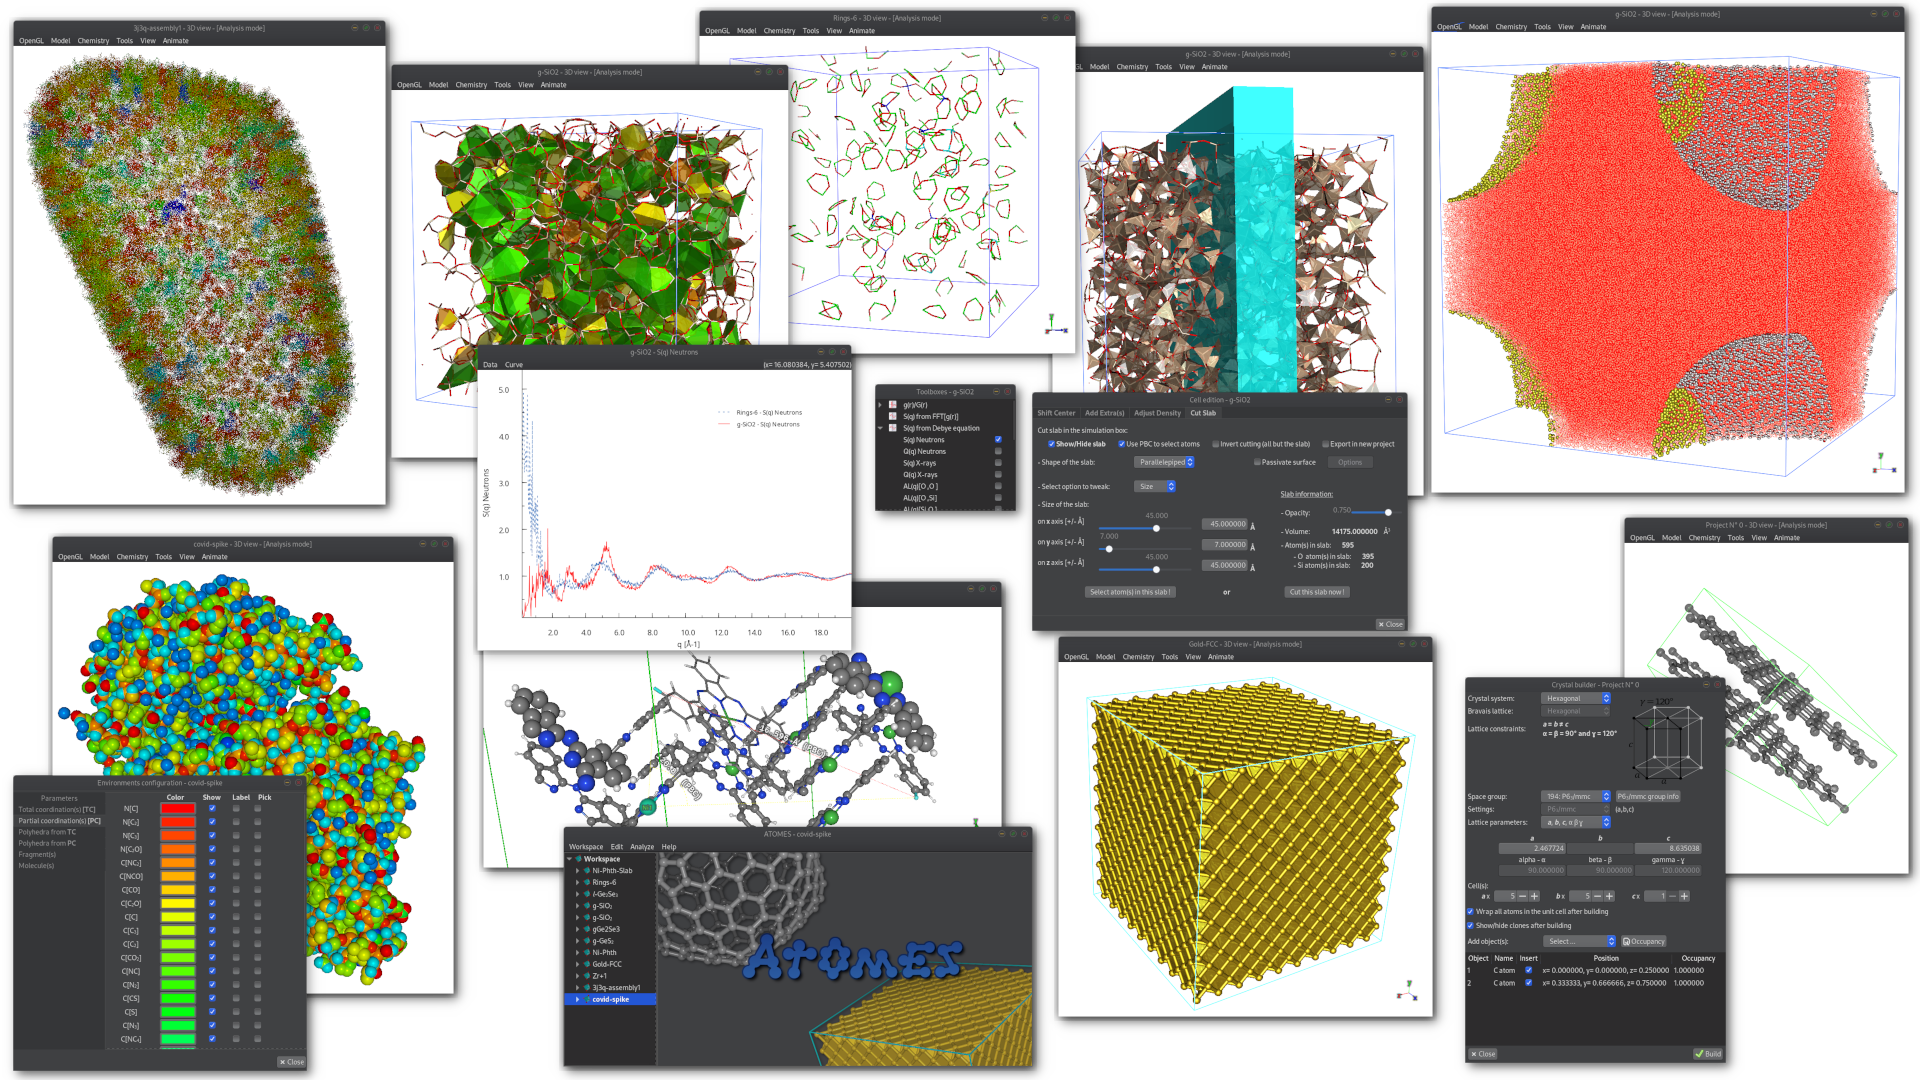
\includegraphics[width=17cm, keepaspectratio=true, draft=\ddst]{img/overview4}\\[0.5cm] \bigskip \atomes: user manual}

\author{Dr. Sébastien {\sc{Le Roux}}\quad\href{mailo:sebastien.leroux@ipcms.unistra.fr}{sebastien.leroux@ipcms.unistra.fr}}
\address{sebastien.leroux@ipcms.unistra.fr}
\universite{Institut de Physique et Chimie des Matériaux de Strasbourg\\
Département des Matériaux Organiques\
BP 43, 23 rue du Loess,\\
F-670234 Strasbourg Cedex 2, France}

\beforepreface

\setcounter{page}{1}            % Je recommence la numerotation a un pour pas
                                % decaler l'alternance droite/gauche et que
                                % les pages impaires soient bien a droite.
%\setcounter{tocdepth}{4}

% Mise en forme TOC/TOF/LOT
{\small \tableofcontents}
\addcontentsline{toc}{chapter}{Contents}
{\it \footnotesize \listoffigures}
\addcontentsline{toc}{chapter}{List of figures}
\chaptermark{List of figures}
{\it \footnotesize \listoftables}
\addcontentsline{toc}{chapter}{List of tables}
\chaptermark{List of tables}

\afterpreface

\vfill                          % Je remplis avec du rien (\vfill}
\pagebreak                      % Je change de page.

%{\small \printindex}

% Intro
\chapter{Introduction}

\atomes\ is a cross-platform Free (Open Source) computational material science tool box. 
It regroups a comprehensive panel of specialized edition tools, several assistants dedicated to the preparation of numerical experiments, 
and, a large number of physico-chemical analysis. 
Advanced visualization utilities and capabilities being available at each stage of the process \atomes\ 
introduces innovative 3D rendering possibilities and intuitive applications of the calculation results. \\[0.25cm]
\atomes\ is designed to analyze, to visualize and to create/edit large three-dimensional atomic scale models, 
and can handle MD trajectories from hundreds of thousands, up to millions, of atoms. 
Using OpenMP parallelization, file processing, coordination and physico-chemical analysis 
make use of the advantages of modern CPUs and their multiple cores. 
Consequently when importing atomic coordinates several properties are analyzed on the fly regardless of the size, 
in number of atoms or MD steps, and the periodicity of the system. \\
\atomes\ offers a workspace that allows to have many projects opened simultaneously. 
The different projects in the workspace can exchange data: analysis results, atomic coordinates ... \\[0.25cm]
\atomes\ also provides an advanced input preparation system for further calculations using well known molecular dynamics codes: 
\begin{itemize}
\item Classical MD : \dlpoly\ \cite{DLPOLY} and \lammps\ \cite{LAMMPS}
\item {\em{ab-initio}} MD : \cpmd\ \cite{CPMD} and \cptk\ \cite{CP2K}
\item QM-MM MD : \cpmd\ \cite{CPMD} and \cptk\ \cite{CP2K}
\end{itemize}
\noindent To prepare the input files for these calculations is likely to be the key, and most complicated step towards MD simulations. 
\atomes\ offers a user-friendly assistant to help and guide the user step by step to achieve this crucial step. 
\begin{figure}[!p]
\hypertarget{overview}{
\begin{center}
\includegraphics*[width=23cm, angle=90, keepaspectratio=true, draft=\ddst]{img/overview4}
\end{center}
\caption{Overview of the \atomes\ program.}\label{overview}
}
\end{figure}


% Programming framework
\chapter{Programming framework}
\label{frame}

\atomes\ is developed in C, GLSL (OpenGL shading language), and  FORTRAN90. 
The \href{https://www.gtk.org/}{GTK} \cite{gtk} library is used to create the {\bf{G}}raphical {\bf{U}}ser {\bf{I}}nterface, and the \href{https://www.openmp.org/}{OpenMP} \cite{OpenMP} API for parallel programming is used to take advantage of the CPU's cores. \\
The 3D rendering is performed, via the \href{https://developer.gnome.org/gtk3/stable/GtkGLArea.html}{GtkGLArea} widget, using modern \href{https://www.opengl.org/}{OpenGL} language \cite{OpenGL},
and the \href{https://github.com/anholt/libepoxy}{Epoxy} library is used to ensure the OpenGL function pointer management. 
Also the  \href{https://www.ffmpeg.org/}{FFmpeg} \cite{ffmpeg} library is used to encode video from off-screen OpenGL rendering. 

\section{Supported platforms}

The \href{https://www.gtk.org/}{GTK} library is a highly portable programming interface which allows \atomes\ to be a cross-platform software. 
Linux, MacOS (Sonoma 14.4.1 - M3 Max processor) and Microsoft Windows (10, 11) versions of the program are available. 

\section{Dependencies and requirements}

\mytable{h}{libs}{
\begin{tabular}{lccc}
\hline
  Library &  & \multicolumn{2}{c}{Version} \\
          &  & Min. required & Recommended \\
\hline
  \href{https://www.gtk.org/}{GTK+}                &             &  3.16 / 4.60 &  3.22 + / 4.60 +\\
  \href{https://www.ffmpeg.org/}{FFmpeg}           &             &   3.1 &  3.41 + \\
  \href{https://github.com/anholt/libepoxy}{Epoxy} &             &   1.3 &  1.43 + \\
  \href{https://www.openmp.org/}{OpenMP}           &             &   4.5 &   4.5 + \\
\hline
\end{tabular}}{Libraries used by \atomes.}{Libraries used by \atomes.}


% Features
\chapter{Features}
\markboth{Features}{\scshape \thesection}

\section{Main window}

\mainfig
The main interface of the \atomes\ program [Fig.~\ref{main}-a] gives access to:
\begin{itemize}
\item The \aob{Workspace menu} [Fig.~\ref{main}-b] to open and save files, including \atomes\ workspace and project files.
\item The \aob{Edit menu} [Fig.~\ref{main}-c] to adjust chemical / physical of a system to be studied/edited.
\item The \aob{Compute menu} [Fig.~ \ref{main}-d] to run some analysis on the \activp\ project (see section \ref{calc} for details).
\item The \aob{Help menu} [Fig.~\ref{main}-e] to access the documentation and a periodic table.
\end{itemize}

\atomes\ allows to build, edit, study, analyse and compare multiple systems within the same instance of the program. 
Each system (molecule(s)/material ...) is defined in a data structure called {\bf{project}}, \atomes\ projects (*.apf files) can be opened/saved separately, 
the list of opened project(s) appears in the left side of the main window in a browsable tree-like structure. 
The entire list of project(s) displayed in this part of the main window is a data structure called {\bf{workspace}}, 
and \atomes\ workspace files (*.awf files) can also be opened and saved, allowing to back up the entire list of projects at once, 
preserving the possible connections, data exchanges, between each projects. \\
An illustration is presented in figure~\ref{overview}, many different projects being opened in the workspace. 
To each of these project is assigned an OpenGL 3D window, few of them being visible in figure~\ref{overview}.  
Double-clicking on the \aob{Workspace} word at the top root of the tree, the list of all projects appears in the right side window. 
This list includes, in bold green font, the name of the \activp\ project (see section~\ref{calc} for details).

\subsection*{Keyboard shortcuts}
\vspace{0.5cm}
\kbdmain
\clearpage

\section{Workspace and project tree}

In \atomes\ each project, as soon as it is created and whether it is new (empty) or contains atomic coordinates, is immediately:
\begin{itemize}
\item inserted into the workspace tree: a branch will appear bearing the project name [Fig.~\ref{ptree}].
\item assigned an OpenGL window for visualization, analysis and edition. 
\item the \aob{Toolboxes} dialog [Fig.~\ref{tools}] is refreshed, and if required open, to present the data of this project.
\end{itemize}
Figure \ref{ptree} illustrates the structure of project tree branch in the \atomes\ workspace. \\
\treefig
\laf On each line/tree branch in the workspace tree the double-click with the left button of the mouse has an effect: 
\begin{itemize}
\item \aob{Workspace} line: displays workspace information, lists all opened project(s) and gives the name of the \activp\ project in bold green font [Fig.~\ref{overview}].
\item \aob{Project's name} line: activates the project (see section~\ref{calc} for details), when the project is \activp\ its name is displayed in bold font.
\item \aob{Settings} line: provides general information about the project.
\item \aob{Visualization} line: open/close the OpenGL visualization window, and display OpenGL/hardware information. 
\item Each of the calculation lines (ex: \aob{g(r)/G(r)}): if the calculation was performed for that project displays summary of the calculation, used parameters, and results. 
\end{itemize}
As illustrated in figure~\ref{wlc} the right click of the mouse display a menu basically reproduces the Workspace menu [Fig.~\ref{main}-b], 
but also introduces two new buttons to activate the project (see section~\ref{calc} for details) and edit its name.\\ 
\myfigure{h}{wlc}{\image{8}{img/p-tree/atomes-wlc}}{Mouse left click menu in the workspace tree of the \atomes\ program.}{Mouse left click menu in the workspace tree of the \atomes\ program.}
\laf The name of the project supports Pango markup\cite{pangomarkup}: \\
\\
{\small{
\begin{tabular}{p{5cm}p{5cm}p{5cm}}
$\bullet$ <sub> </sub> for $_{\text{underscore}}$ & $\bullet$ <i> </i> for {\it{italic}} & $\bullet$ <u> </u> for {\uline{underline}} \\[0.25cm]
$\bullet$ <sup> </sup> for $^{\text{exponent}}$ & $\bullet$ <b> </b> for {\bf{bold}} & $\bullet$ <tt> </tt> for {\texttt{monospace}} \\[0.25cm]
\multicolumn{3}{l}{and more ... see: \href{https://docs.gtk.org/Pango/pango\_markup.html}{https://docs.gtk.org/Pango/pango\_markup.html}}\\[0.25cm]
\end{tabular}
}}

\section{Files}

\subsection{Importing atomic coordinates}
\label{import}

The list of the supported format of atomic coordinates is presented in appendix~\ref{inout}. \\ 
\href{https://isaacs.sourceforge.net}{ISAACS} files contains all the information required to prepare analysis and visualization. 
For the other file formats, and after reading the atomic coordinates, dialog boxes appears automatically in the following order:
\subsubsection*{1) The \aob{Chemistry and physics} dialog [Fig.~\ref{cpd}]}
\myfigure{h}{cpd}{\image{8}{img/main/atomes-cpd}}
{The \aob{Chemistry and physics} dialog in the \atomes\ program.}{The \aob{Chemistry and physics} dialog in the \atomes\ program.}
This dialog allows to tweak the chemical and physical properties of the elements found in the coordinates file (see figure~\ref{cpd}). \\
Particular attention should be given to the selection of the neutrons and X-rays scattering length, 
for the former parameters are included in \atomes\ (see chapter~\ref{datab}), 
for the latter two possibilities are offered to the user:
\begin{itemize}
\item Use the exact Q dependent method to compute X-rays S(Q) related properties.
\item Use an approximation with the X-rays scattering length equal to the atomic number of the element.
\end{itemize}
%\clearpage
\subsubsection*{2) The \aob{Box and periodicity} dialog [Fig.~\ref{bpd}]}
\bpdfig
This dialog allows to define the periodicity and if needed adjust the model box proportions, or lattice vectors (see [Fig.~\ref{bpd}]). 
\subsubsection*{3) The \aob{Bond cutoffs} dialog [Fig.~\ref{bcd}]}
\myfigure{h}{bcd}{\image{8}{img/main/atomes-bcd}}{The \aob{Bond cutoffs} dialog in the \atomes\ program.}{The \aob{Bond cutoffs} dialog in the \atomes\ program.}
This dialog allows to adjust the cutoff distances used to define the existence or absence of chemical bonds (see figure~\ref{bcd}), 
both for the calculations (see section~\ref{calc}) sensitive to these parameters and for the 3D visualization in the OpenGL window (see section~\ref{visu}). \\ 
%\clearpage
As soon as the \aob{Bond cutoffs} dialog closes \atomes\ will have everything required to setup the 3D model and the OpenGL window will appear. \\
\\
The 3 dialog boxes \aob{Chemistry and physics}, \aob{Box and periodicity} and \aob{Bond cutoffs} can be re-opened again later on using the \aob{Edit} menu [Fig.~\ref{main}-c]. 
However in that case only the \activp\ project parameters can to be modified. Therefore remember to activate the project you want to edit before using the edit menu.
\clearpage

\subsection{Reading \atomes\ project file(s)}
\label{apf}

The \atomes\ project file allows to store:
\begin{itemize}
\item The atomic coordinates, including MD trajectories.
\item The results/data of all calculations performed within \atomes. 
\item The results of all modifications of the calculations data, including graph windows (see chapter~\ref{ana}). 
\item The parameters of the OpenGL window, so that when re-opened the project appears exactly as it was when saved. 
\end{itemize}
The main idea being to be able to resume work exactly where it was before saving the \atomes\ project file. \\
\\The \atomes\ project files have the extension: {\bf{.apf}} \\
\\
To open \atomes\ project file(s) use the \aob{Open Project File(s)} dialog [Fig.~\ref{oapf}]. \\
This can be done using alternatively: 
\begin{itemize}
\item The workspace menu.
\item The right click menu obtained with the mouse button of the workspace tree.
\item The keyboard shortcut \Ctrl + \keystroke{o} on top of the \atomes\ program main window.
\end{itemize}
Many \atomes\ project files can be opened simultaneously, simply select all projects to be opened in the \aob{Open Project File(s)} dialog, click \aob{Open} and they will appear in the workspace tree: \\
\oapfig
\laf Later on when using the \atomes\ program remember that any window specifically dedicated to a project will have the name of this project in its title bar. 
\clearpage

\subsection{Reading \atomes\ workspace file(s)}
\label{awf}

The \atomes\ workspace file allows to store:
\begin{itemize}
\item A collection of \atomes\ projects. 
\item The relations between these projects, data exchanges, comparisons ...
\end{itemize}
Again the idea is to be able to resume work exactly where it was before saving the \atomes\ workspace file. \\
\\The \atomes\ workspace files have the extension: {\bf{.awf}}\\
\\
To open \atomes\ workspace file use the \aob{Open Workspace} dialog [Fig.~\ref{owpf}]. \\
This can be done using alternatively: 
\begin{itemize}
\item The workspace menu.
\item The right click menu obtained with the mouse button of the workspace tree.
\item The keyboard shortcut \Ctrl + \keystroke{w} on top of the \atomes\ program main window. 
\end{itemize}
Only a single \atomes\ workspace file can be opened at a time, if needed close the opened workspace, then open the new one: 
\owpfig

\clearpage

\section{Analyzing models using \atomes}
\label{calc}

\atomes\ can compute the following structural characteristics of a 3D structure model:
{\small{
\begin{itemize}
\item Radial distribution functions g(r) (RDFs) \cite{AlTilde} including $^{\circ}$:
\begin{itemize}
\item Total RDFs for neutrons and X-rays.
\item Partial RDFs.
\item Bhatia-Thornton RDFs \cite{2007JNCS..353.2959S}
\end{itemize}
$^{\circ}$ Radial distribution functions can be computed by i) direct real space calculation and/or ii) Fourier transforming of the structure factor calculated using the Debye formalism \cite{EurJM.14-233.2002}
\item Structure factors S(q) \cite{EurJM.14-233.2002} including $^{\circ\circ}$:
\begin{itemize}
\item Total structure factors S(q) for neutrons and X-rays.
\item Total Q(q) \cite{EurJM.14-233.2002,jac.17-61.1984} for neutrons and X-rays.
\item Partial S(q):
\begin{itemize}
\item Faber-Ziman \cite{PhilMag.11.153} partial S(q)
\item Ashcroft-Langreth \cite{PhysRev.156.685,PhysRev.159.500,PhysRev.166.934.2} partial S(q)
\item Bhatia-Thornton \cite{PhysRevB.2.3004} partial S(q)
\end{itemize}
\end{itemize}
$^{\circ\circ}$ Structure factors can be computed by i) Fourier transforming of the radial distribution functions and/or ii) using the Debye formalism \cite{EurJM.14-233.2002}
\item Interatomic bond properties
\begin{itemize}
\item Coordination numbers
\item Atomic near neighbor distribution
\item Fraction of links between tetrahedra
\item Fraction of tetrahedral units
\item Bond lengths distribution for the first coordination sphere
\end{itemize}
\item Distribution of Bond angles
\item Distribution of Dihedral angles
\item Ring statistics, according to several definitions:
\begin{itemize}
\item All closed paths (no rules)
\item King's rings \cite{Nature.213.1112,PhysRevB.44.4925}
\item Guttman's rings \cite{Guttman-116-145}
\item Primitive rings \cite{Goetzke-127.215,YuanCormack-24-343} (or Irreducible \cite{Wooten-bk0109})
\item Strong rings \cite{Goetzke-127.215,YuanCormack-24-343}
\end{itemize}
And including options to:
\begin{itemize}
\item search only for ABAB rings
\item exclude rings with homopolar bonds (A-A or B-B) from the analysis
\end{itemize}
Ring statistics is presented according to the R.I.N.G.S. method \cite{RINGS}.
\item Chain statistics, including options to:
\begin{itemize}
\item search only for AAAA chains
\item search only for ABAB chains
\item exclude chains with homopolar bonds (A-A or B-B) from the analysis
\item search only for 1-(2)$_n$-1 chains
\end{itemize}
\item Spherical harmonics invariant, $Q_l$, as local atomic ordering symmetry identifiers \cite{PhysRevB.28.784}
\begin{itemize}
\item Average Q$_l$ for each chemical species
\item Average Q$_l$ for a user specified structural unit
\end{itemize}
%\item Bond valence sums \cite{BondValence, ActaCryst.B41.244, ActaCryst.A29.266}
%\begin{itemize}
%\item Average bond valence for each chemical species
%\item Average bond valence for a user specified structural unityelke
%\end{itemize}
\item Mean Square Displacement of atoms (MSD)
\begin{itemize}
\item Atomic species MSD
\item Directional MSD (x, y, z, xy, xz, yz)
\item Drift of the center of mass
\end{itemize}
\end{itemize}
}}
See appendix \ref{physics} to learn more about the physics and the chemistry behind these calculations. \\
\\
The calculations presented in this list can only be performed on the \activp\ project, ie. the project which 
name appears in the title bar of the \atomes\ program main window, in bold font in the \atomes\ workspace tree and in green bold font in the workspace information dialog [Fig.~\ref{overview}]. \\
For more about running calculation using \atomes\ see chapter~\ref{ana}.

\clearpage

\section{Visual analysis using \atomes}
\label{visu}

Each model in the \atomes\ workspace is assigned an OpenGL window that provides an interactive experience to visualize and analyze its properties. 
Isolated configurations as well as entire molecular dynamics trajectories can be visualized. \\ 
Among the possibilities of the OpenGL window: 
\begin{itemize}
\item Advanced color map options, for both atoms and polyhedra. 
\item Advanced coordination(s) visualization options (total, partial, fragments, molecules). 
\item Advanced coordination polyhedra visualization options. 
\item Measurement tools.
\item Advanced layout system for atomic labels, measurements, MD box and model axis. 
\item Image and movie rendering, including an intuitive interface to movie encoding that allows to record every interaction/modification made to the OpenGL window. 
\item Advanced OpenGL configuration options.
\end{itemize}
For a complete description of these features see chapter~\ref{visual}. 

\section{Visual edition and model creation using \atomes}
\label{edit}

Using \atomes\ \aob{Crystal builder} it is possible to build crystalline structures or even super-structures.  
Also if the model description contains a box, then cell edition options become available:
\begin{itemize}
\item Wrap atoms in original cell
\item Shift cell center
\item Add extra cell(s)
\item Create super cell
\item Change the model density
\item Cut slabs or extract atoms from the model.
\end{itemize}
And if the model contains only a single configuration (and not a molecular dynamics trajectory), or when an empty project is created, the atom(s) edition options/mode become available:
\begin{itemize}
\item Motion (random or selected atom(s))
\item Replacement (random or selected atom(s))
\item Removal (random or selected atom(s))
\item Insertion
\end{itemize}
For a complete description of these features see chapter~\ref{edition}.

\section{Preparing MD calculations in \atomes}

\atomes\ provides input creation assistants for well known molecular dynamics codes:
\begin{itemize}
\item \cpmd\ \cite{CPMD}
\item \cptk\ \cite{CP2K}
\item \dlpoly\ \cite{DLPOLY}
\item \lammps\ \cite{LAMMPS}
\end{itemize}
For a complete description of these features see chapter~\ref{md}.



% PC analysis
\include{chap-4/chap-4}

% Vis analysis
\chapter{Visual analysis in \atomes}
\markboth{Visual analysis in \atomes}{\scshape \thesection}
\label{visual}

In this chapter examples will be illustrated using an \atomes\ workspace presented in figure~\ref{workm}, this workspace contains 3 different projects:
\begin{itemize}
\item a molecular surface of Nickel-Phthalocyanine molecules with 512 atoms.
\item a \sio\ glass with 3000 atoms. 
\item a \ges\ glass molecular dynamics trajectory with 500 MD steps and 258 atoms.
\end{itemize}
\myfigure{h}{workm}{\hspace{-2cm}\image{15.5}{img/visu/workm2}}{Example workspace: visualization.}
{Example workspace to illustrate the visualization capabilities of the \atomes\ program containing 3 projects, named \mbox{\aob{Ni-Phth}}, \aob{g-\sio} and \aob{l-\ges}.}

\section{Window top bar menu}

In order to present the functionalities available in the OpenGL window, we will browse the top bar menu [Fig.~\ref{workm}] and present each submenu one after the other. \\
%\myfigure{h}{\image{10}{img/visu/glwin_top}}{The top bar menu of the OpenGL window in the \atomes\ program.}
% {The top bar menu of the OpenGL window in the \atomes\ program.}

\subsection{The \aob{OpenGL} menu}

\moglfig

The \aob{OpenGL} menu is detailed in figure~\ref{mogl}. The behavior of the \aob{Render} menu [Fig.~\ref{mogl}-c], and the \aob{Quality} menu [Fig.~\ref{mogl}-d], 
as well as of the \aob{Render image} button being pretty intuitive the following only detail the behavior of the \aob{Style menu}, 
the \aob{Color scheme(s)} menu [Fig.~\ref{mogl}-b], and the \aob{Material and lights} button.

\clearpage
\subsubsection{The \aob{Style} menu}
\label{stylem}

Using the \aob{Style} menu it is possible to define to {\bf{default style}} of the model representation, the options are among the most commonly used in chemistry. 
Changing the {\bf{default style}} from this menu will update several parts of the OpenGL window and associated menus. 
For instance selecting the \aob{Ball and stick} option will update the first tab of \aob{Atom(s) configuration} dialog [Fig.~\ref{advats}] to display atomic radius 
and the \aob{Bond(s)} menu [Fig.~\ref{modl}] to present the \aob{Radius(ii)} and offer a shortcut to modify their values. \\
It is possible to define local style(s) to improve the visual representation, however this is only possible using the mouse, see section~\ref{mstyle}, 
and changing the {\bf{default style}} of the model using the \aob{Style} menu will reset/erase any local style(s) value(s) to the default. 

\subsubsection{The \aob{Color scheme(s)} menu}
\label{csm}

In the \atomes\ program when the file is opened most of the bonding properties are calculated "on-the-fly", allowing to gain insights on the atomic coordinations, 
as well as the number of fragments and the different molecules in the model. \\
Therefore before using the \aob{Color scheme(s)} menu it is important to be familiar with the following definitions: 
\begin{itemize}
\item {\bf{Total coordination}} = total number of first neighbor atoms around the atom.
\item {\bf{Partial coordination}} = number of atoms of each chemical species around the atom.
\item {\bf{Fragments}} = isolated molecular objects in the model. 
\item {\bf{Molecules}} = the different topological objects in the model.
\item {\bf{Coordination polyhedra}} = structure drawn by linking the atoms of the first coordination sphere for a particular atom. 
Requires the considered atom to have 3 neighbors, then the atom it-self is used as a point to build the polyhedra, or more.
\end{itemize}
The \aob{Color scheme(s)} menu allows to change the Color Map (CM) for both atoms and coordination polyhedra, 
based on the bonding analysis performed using the bond cutoff(s) specified by the user. 
An illustration is provided in figure~\ref{cmaps} for the \aob{Ni-Phth} project of the example workspace, 
note that is this model the molecule on the top is missing a hydrogen atom compared to the one that composed the surface. \\
The colors of each objects can be modified/adapted via the appropriate menus/dialogs (see sections~\ref{modelm} and \ref{chemm}). \\ 
\cmapfig

\clearpage

\subsubsection*{Using a custom color map}

Alternatively to the CMs proposed by the \atomes\ program it is possible to apply a user defined CM to the OpenGL model, 
this option is accessible via the \aob{Custom} button of the \aob{Atoms \& bonds} menu [Fig.~\ref{mogl}-b]. 
In that case it is required to read a file (having the extension "*.dat") that contains the numerical data to be used as color scale. 
This file must be a simple (Unix like) text file with as many lines as: 
\begin{center}{\bf{Total number of MD steps $\times$ Total number of atoms}}\end{center} 
Indeed the new colors can be applied to the entire MD trajectory. \\
An example is provided hereafter for the silica glass model: \\
\begin{enumerate}
\item In the initial setup the chemical species are used as color map:
\begin{center}\image{12}{img/visu/cmap/sio2-init}\end{center}
\item When the \aob{Custom} button is pressed for the atoms CMs, the \aob{Custom color map setup} dialog appears: 
\begin{center}\image{6}{img/visu/cmap/custom}\end{center}
\item {\bf{(a)}} The \aob{Import / Save data} button allows to import your data file to create the color map. 
If the data file is processed successfully then \atomes\ will propose to use it and a confirmation dialog will pop-up: 
\begin{center}\image{8}{img/visu/cmap/custom-read}\end{center}
For this example the data points are simply the atom indices from 1 to 3000. 
\item {\bf{(b)}} Afterwards using the \aob{Edit data} button it becomes possible to edit the data in a basic spreadsheet like mode, 
so that values for a particular atom can be checked and/or modify if needed:
\begin{center}\image{5}{img/visu/cmap/custom-edit}\end{center}
\item {\bf{(c)}} And using the \aob{Customize color map} button is possible to customize the color map, 
initially a gradient of red an blue between the maxima and the minima of the values in the data set is used, 
but you can easily add or remove point(s), and adjust the corresponding color to enhance the visual representation of your model: 
\begin{center}
\hspace{-2cm}
\begin{tabular}{cp{3cm}c}
\image{7}{img/visu/cmap/custom-cinit} & \multicolumn{1}{c}{\raisebox{5cm}{$\Longrightarrow$}} &
\image{7}{img/visu/cmap/custom-cmore}
\end{tabular}
\end{center} 
\item Finally simply apply the changes to use the new colors:
\begin{center}\image{14}{img/visu/cmap/sio2-custom}\end{center}
\item The \aob{Custom} data and the corresponding color map are saved within the \atomes\ project and workspace files (see section~\ref{apf} and \ref{awf}), 
so that it will not be require to load a prepare the color map between work sessions.
\end{enumerate}
  
%\image{5}{img/visu/cmap/custom-init} \\
%\image{8}{img/visu/cmap/custom-read} \\
%\image{5}{img/visu/cmap/custom-ok} \\
%\image{6}{img/visu/cmap/custom-edit} \\
%\image{7}{img/visu/cmap/custom-cinit} \\
%\image{7}{img/visu/cmap/custom-cmore}

\subsubsection{Material and lights}

The \aob{Material and lights} button of the \aob{OpenGL} menu opens the \aob{OpenGL material aspect and light settings} dialog [Fig.~\ref{advogl}]:\\
\myfigure{h}{advogl}{\image{17}{img/visu/adv-ogl}}{The \aob{OpenGL material aspect and light settings} dialog in the \atomes\ program.}
{The \aob{OpenGL material aspect and light settings} dialog in the \atomes\ program.}
\laf The window contains a notebook with 3 tabs:
\begin{itemize}
\item The first tab allows to configure/adjust:
\begin{itemize}
\item The quality of the rendering, ie. the number of polygons to render a volume. 
\item The lightning model, from the lowest quality (fastest to render, \aob{None}) to the highest quality (longer to render, \aob{Cook-Torrance-GCX}).
\item The material aspect, few templates being available, but all characteristics required to describe the material aspect for the light mode being available. 
\end{itemize}
\item The second tab allows to configure the lights sources of the model: 
\begin{itemize}
\item 3 type of light source being available: directional, point and spot lights.
\item With the possibility to add up to 10 light sources. 
\end{itemize}
\item Finally the third tab is used to adjust the fog effects 
\end{itemize}
For information on OpenGL lightning models, material effects, lights, and more see: 
\begin{itemize}
\item \href{https://learnopengl.com/Lighting/Basic-Lighting}{https://learnopengl.com/Lighting/Basic-Lighting}
\item \href{https://learnopengl.com/Advanced-Lighting/Advanced-Lighting}{https://learnopengl.com/Advanced-Lighting/Advanced-Lighting}
\end{itemize}

\clearpage

\subsection{The \aob{Model} menu}
\label{modelm}
\vspace{-0.25cm}
\modlfig

\clearpage

\subsubsection{The \aob{Atom(s)} menu}

The \aob{Atom(s)} menu [Fig.~\ref{modl}-a] offers to configure some visual features related to the chemical species in the model. 
This menu contains shortcuts for some the properties that can be adjusted using the more advanced \aob{Atom(s) configuration} dialog, 
and that can be opened using any of the \aob{Advanced} buttons in the menu. 
The \aob{Atom(s) configuration} dialog is presented in figure~\ref{advats}:
\myfigure{h}{advats}{\image{17}{img/visu/atom-adv}}
{The \aob{Atom(s) configuration} dialog in the \atomes\ program.}{The \aob{Atom(s) configuration} dialog in the \atomes\ program.}
\laf The window contains a notebook with 3 tabs:
\begin{itemize}
\item {\bf{(a)}} The \aob{Display  properties} tab: to adjust chemical species colors, atomic labels, and depending on the model style: 
\begin{itemize}
\item Ball and sticks: atomic radius
\item Wireframe or Points: point size
\end{itemize}   
\item {\bf{(b)}} The \aob{Label properties} tab: to adjust the aspect of the atomic labels.
\item {\bf{(c)}} or {\bf{(d)}} The \aob{Atom(s) selection}: to search for atom(s) in the model. 
If the model contains less than 10 000 atoms the entire list of atoms is displayed {\bf{(c)}}, 
otherwise it becomes too complicated to display and a search engine is proposed {\bf{(d)}}.
\end{itemize}

\clearpage

\subsubsection{The \aob{Bond(s)} menu}  

Via the \aob{Bond(s)} menu [Fig.~\ref{modl}-b] it is possible to adjust the bond cutoff(s), and depending on the model style:
\begin{itemize}
\item Ball and sticks: bonds radius(ii)
\item Cylinders: bond radius
\item Wireframe: line width
\end{itemize}

\subsubsection{The \aob{Clone(s)} menu}
\label{Clones}

The \atomes\ program uses {\bf{clones}} to illustrate the presence of atomic bond(s) on the edges of the simulation box and 
existing because of the periodic boundary conditions (see section~\ref{pbc} for more information on the PBC). \\ 
For the \aob{Clone(s)} menu to be activated two conditions must be fulfilled: to use PBC, ie. the model must have a periodicity, and, for such bonds via PBC to exist. 
If both conditions are met, then the first button of the menu to \aob{Show/Hide Clones} will be active and it becomes possible to show or hide the {\bf{clones}}. \\ 
Please note that {\bf{clone}} atoms/bonds are translucent to make them easily distinguishable from their atom/bond counterparts, 
figure~\ref{atcl} illustrates the {\bf{clones}} idea using the silica glass model:
\clonefig
\laf If the {\bf{clones}} are visible then the two \aob{Atom(s)} and \aob{Bond(s)} submenus will be activated as well.
These menus are reproductions of the upper level \aob{Atom(s)} and \aob{Bond(s)} menus, and windows, but dedicated to the {\bf{clones}}, 
this allows to make the {\bf{clones}} even more distinguishable in the 3D representation. 

\clearpage

\subsection{The \aob{Chemistry} menu}
\label{chemm}

\vspace{-0.5cm}
\mchemfig

The \aob{Chemistry} menu [Fig.~\ref{mchem}] and all the attached submenus from {\bf{a)}} to {\bf{e)}} are essentially composed of shortcut buttons to the options/actions that can be performed using the \aob{Environments configuration} window, this section will therefore focus on the presentation of this window. 

\subsubsection*{The \aob{Environments configuration} window}
\label{ecw}

The \aob{Environments configuration} window contains a notebook with several tabs. 
The number of tabs depends on the calculations that were performed to analyze the model, 
ring statistics and chain statistics calculations will insert new tabs in the notebook. 
The different tabs of \aob{Environments configuration} window are:
\begin{enumerate}
\item\label{t:1} The \aob{Parameters} tab  (see \ref{show t:1})
\item\label{t:2} The \aob{Total coordination(s) [TC]} tab (see \ref{show t:2/3})
\item\label{t:3} The \aob{Partial coordination(s) [PC]} tab (see \ref{show t:2/3})
\item\label{t:4} The \aob{Polyhedra from TC} tab (see \ref{show t:4/5})
\item\label{t:5} The \aob{Polyhedra from PC} tab (see \ref{show t:4/5})
\item\label{t:6} The \aob{Fragment(s)} tab (see \ref{show t:6/7})
\item\label{t:7} The \aob{Molecule(s)} tab (see \ref{show t:6/7})
\item\label{t:8} The \aob{{\em{? ring(s)}} [{\em{?R}}]} tab (see \ref{show t:8a} and \ref{show t:8b})\\
\qquad The \aob{Polyhedra from [{\em{?R}}]} tab \\
\qquad The \aob{Isolated ring(s) from [{\em{?R}}]} tab
\item\label{t:9} The \aob{Chain(s)} tab (see \ref{show t:9})\\
\qquad The \aob{Isolated chain(s)} tab
\end{enumerate}
Tabs~\ref{t:1}, \ref{t:2}, \ref{t:3}, \ref{t:4} and \ref{t:5} are always present in the notebook, 
tabs~\ref{t:6} and \ref{t:7} are present providing that the fragment(s) and the molecule(s) analysis were performed.  
Tabs~\ref{t:8} are inserted in the notebook when any of the ring statistics analysis are completed, whereas the tabs~\ref{t:9} are inserted when the chain statistics analysis is completed. 
Overall the \aob{Environments configuration} window can contain up to 24 tabs.\\
Each tab in [\ref{t:1}-\ref{t:9}] is presented in detail thereafter: 
\clearpage
\newcommand{\cosize}{8.0}
\begin{enumerate}
\item\label{show t:1} {\bf{The \aob{Parameters} tab}}
\begin{center}\image{\cosize}{img/visu/wcoord/wcoord-p}\end{center}
This tab reproduce this available color map options from the \aob{Color scheme(s)} menu (see section~\ref{csm}). 
Many of the following tabs allow to adjust the color of the element(s) for each color map, only for the change to be visible the corresponding color map must be used. \\
The \aob{Parameters} tab also contains a \aob{Cloned polyhedra} button, that allows to display polyhedra on the edges of the simulation box, and this even if {\bf{clones}} are not shown.
\clearpage
\item\label{show t:2/3} {\bf{The \aob{Total coordination(s) [TC]} and \aob{Polyhedra form TC} tabs}} \\[0.5cm]
\begin{tabular}{lcp{0.25cm}lc}
\hspace{-2.5cm} {\bf{a)}} & & & {\bf{b)}} \\
\hspace{-2.5cm} & \image{\cosize}{img/visu/wcoord/wcoord-tc} & & &
 \image{8}{img/visu/wcoord/wcoord-ptc} 
\end{tabular}
\\[0.25cm]
{\bf{a)}} The \aob{Total coordination(s) [TC]} tab presents a list of options related to the total coordination sphere(s)
found during the bonding analysis:
\begin{itemize}
\item A \aob{Color} button: to adjust the color of the each element. Initially a color being assigned to each number of neighbors independently of the chemical species involved. 
\item A \aob{Show} button: to hide/show the atom(s) matching the associated property.
\item A \aob{Label} button: to hide/show the atomic label of the atom(s) matching the associated property.
\item A \aob{Pick} button: to select/unselect the atom(s) matching the associated property (for more information on atom selection see section~\ref{mviz}) .
\end{itemize}
In the \aob{Ni-Phth} project example, the colors in {\bf{a}} allow to obtain the representation from [Fig.~\ref{cmaps}-a]. \\ 
{\bf{b)}} The \aob{Polyhedra form TC} tab presents a list of options related to the total coordination sphere(s) with 3 or more neighbors:
\begin{itemize}
\item An \aob{Alpha} range: to adjust the opacity of the coordination polyhedra for the atom(s) matching the associated property.
\item A \aob{Show} button: to hide/show the coordination polyhedra for the atom(s) matching the associated property.
\end{itemize}
\clearpage
\item\label{show t:4/5} {\bf{The \aob{Partial coordination(s) [PC]} and \aob{Polyhedra form PC} tabs}} \\[0.25cm]
\begin{tabular}{lcp{0.25cm}lc}
\hspace{-2.5cm} {\bf{c)}} & & & {\bf{d)}} \\
\hspace{-2.5cm} & \image{\cosize}{img/visu/wcoord/wcoord-pc} & & &
 \image{8}{img/visu/wcoord/wcoord-ppc} 
\end{tabular}
\\[0.25cm]
The \aob{Partial coordination(s) [PC]} {\bf{c)}} and the \aob{Polyhedra form PC} {\bf{d)}} tabs are similar to {\bf{a)}} and {\bf{b)}} respectively, 
coordination spheres being also separated based on the analysis of the chemistry of the bond(s). 
In the \aob{Ni-Phth} project example, the colors in {\bf{c)}} allow to obtain the representation from [Fig.~\ref{cmaps}-b].
\item\label{show t:6/7} {\bf{The \aob{Fragment(s)} and \aob{Molecule(s)} tabs}} \\[0.25cm]
\begin{tabular}{lcp{0.25cm}lc}
\hspace{-2.5cm} {\bf{e)}} & & & {\bf{f)}} \\
\hspace{-2.5cm} & \image{\cosize}{img/visu/wcoord/wcoord-frag} & & &
\image{\cosize}{img/visu/wcoord/wcoord-mol} 
\end{tabular}
\\[0.25cm]
The \aob{Fragment(s)} {\bf{e)}} and \aob{Molecule(s)} {\bf{f)}} tabs follow similar ideas than {\bf{a)}} (or {\bf{c)}}) but for the {\bf{fragment(s)}} and {\bf{molecule(s)}} respectively. 
In these examples from the \aob{Ni-Phth} project, the colors in {\bf{e)}} and {\bf{f)}} allow to obtain respectively the representations from [Fig.~\ref{cmaps}-c] and [Fig.~\ref{cmaps}-d].
\clearpage
\item\label{show t:8a} {\bf{The \aob{{\em{? ring(s)}} [{\em{?R}}]}, \aob{Polyhedra from [{\em{?R}}]} tabs}}\\[0.5cm]
\begin{tabular}{lcp{0.25cm}lc}
\hspace{-2.5cm} {\bf{g)}} & & & {\bf{h)}} \\
\hspace{-2.5cm} & \image{\cosize}{img/visu/wcoord/wcoord-kr} & & &
\image{\cosize}{img/visu/wcoord/wcoord-pkr} 
\end{tabular}
\\[0.25cm]
Whenever a ring statistics calculation is performed successfully and ring(s) is/are found in the model, 
the \aob{{\em{? ring(s)}} [{\em{?R}}]} {\bf{g)}} and \aob{Polyhedra from [{\em{?R}}]} {\bf{h)}} tabs are inserted in the \aob{Environments configuration} window, 
{\bf{g)}} and {\bf{h)}} are examples from the g-\sio\ model for which King's rings analysis was performed. 
If other analyses were performed more tabs would be inserted following a similar idea, and {\bf{?}} is the name of the methodology to search for rings, 
among: All (No rules), King's, Guttman's, Primitive and Strong (see section~\ref{rstat} for more information on ring statistics). \\
The \aob{{\em{? ring(s)}} [{\em{?R}}]} tab presents a list of options related results of the ring statistics calculation, for each size of ring:
\begin{itemize}
\item A \aob{Color} button: to adjust the color of the each element. Note that this color only concerns the polyhedra. 
Initially a different color is assigned to each size of ring(s).
\item A \aob{Show} button: to hide/show the atom(s) involved in ring(s) of that size.
\item A \aob{Label} button: to hide/show the atom(s) involved in ring(s) of that size.
\item A \aob{Pick} button: to select/unselect the atom(s) involved in ring(s) of that size.
\end{itemize}
The \aob{Polyhedra from [{\em{?R}}]} tab present other options related results of the ring statistics calculation, for each size of ring:
\begin{itemize}
\item An \aob{Alpha} range: to adjust the opacity of the polyhedra drawn using the atom(s) of each ring of that size as summits.
\item A \aob{Show} button: to hide/show the polyhedra drawn using the atom(s) of each ring of that size as summit.
\end{itemize}
\clearpage
\item\label{show t:8b}{\bf{The \aob{Isolated ring(s) from [{\em{?R}}]} tab}} \\
\begin{tabular}{lcp{0.25cm}lc}
\hspace{-2.5cm} {\bf{i)}} & & & {\bf{j)}} \\
\hspace{-2.5cm} & \image{\cosize}{img/visu/wcoord/wcoord-akr-a} & & &
\image{\cosize}{img/visu/wcoord/wcoord-akr-b} 
\end{tabular}
\\[0.25cm]
In the \aob{Isolated ring(s) from [{\em{?R}}]} tab every single ring found can be look-up individually. 
Most often {\bf{i)}} version of the tab is used, however if more than 10 000 rings are found 
it becomes too complicated to display the entire list and a search engine is proposed instead {\bf{j)}}. \\
Among the options provided by the  \aob{Isolated ring(s) from [{\em{?R}}]} tab:
\begin{itemize}
\item A \aob{Show} button: to hide/show the atom(s) involved in this ring.
\item A \aob{Ploy} button: to hide/show the polyhedra drawn using the atom(s) of this ring as summits.
\item A \aob{Label} button: to hide/show the atom(s) involved in this ring.
\item A \aob{Pick} button: to select/unselect the atom(s) involved in this ring.
\end{itemize}
\item\label{show t:9} {\bf{The \aob{Chain(s)} \aob{Isolated chain(s)} tabs} }\\[0.25cm]
These tabs (not shown) are dedicated to the results of the chain statistics analysis, and simply reproduces options of tabs {\bf{g)}} and {\bf{i)}}/{\bf{j)}},
at the exception that there are no polyhedra to display. 
\end{enumerate}
\clearpage

\subsection{The \aob{Tools} menu}

\mtoolfig
The \aob{Edit} menu {\bf{a)}}, that regroups the edition tools will be covered in chapter~\ref{edit}, and the \aob{Molecular Dynamics} menu {\bf{d)}},
regrouping the MD input assistants will be covered in chapter~\ref{md}. Also the actions of the \aob{Invert} menu {\bf{e)}} being pretty intuitive, 
this section will only present the \aob{Measures} button/dialog, the \aob{Mouse mode} {\bf{b)}}, \aob{Selection mode} {\bf{c)}} menus. 

\subsubsection*{The \aob{Measures} dialog}
\label{mdw}

Pressing the \aob{Measures} button will open the \aob{Measures} dialog [Fig.~\ref{mdial}], that contains a notebook with 3 tabs, for inter-atomic distances, angles and dihedrals, 
and a button labelled \aob{Font and style} to configure how the measure(s) will appear on the model. \\ 
\myfigure{h}{mdial}{
%\begin{tabular}{lclclc}
%\hspace{-2cm} {\bf{a)}} & & {\bf{b)}} & & {\bf{c)}} \\
%\hspace{-2cm}  & \image{5.5}{img/visu/wmeas/bonds} &
%  & \image{5.5}{img/visu/wmeas/angles} &
%  & \image{5.5}{img/visu/wmeas/dih}
%\end{tabular}
\hspace{-1cm} \image{17.5}{img/visu/wmeas/meas}}
{The \aob{Measures} dialog in the \atomes\ program.}{The \aob{Measures} dialog in the \atomes\ program, with the \aob{Distances}, \aob{Angles} and \aob{Dihedrals} tabs.}
\laf Each tab contains the respective measured properties for all the atoms in selection (see section~\ref{mviz} for more information on the selection process), 
this means the atoms that have been selected before opening the dialog, or, while it is opened and the tabs will refresh. 
The tabs read as follow: 
\begin{itemize}
\item First (2/3/4) columns the atoms id's
\item Column (3/4/5): the value measured in the model
\item Column (4/5/9): If PBC are used/required to measure the value (to avoid visual deception) 
\end{itemize}
\clearpage
{\bf{Behavior of the \aob{Measures} dialog:}}
\begin{enumerate}
\item If too many atoms are in selection then the tabs will remain empty and the measures will not show up. 
To get the information about the measures back simply decrease the number of atoms selected under 20 atoms for the distances and the angles, and under 10 for the dihedrals. \\
\item If any line is selected by a mouse click in the tabs, then the font color of this line will change and the corresponding measure will appear in the model with the same color. 
In figure~\ref{mdial}, 2 lines are selected in the \aob{Distances} tab, and 1 line is selected in the \aob{Angles} tab, the result is presented in figure~\ref{ex-meas}. \\
\myfigure{h}{ex-meas}{\image{15}{img/visu/wmeas/Ni-Phth-meas2}}{Some examples of measurements displayed in the OpenGL window.}{Some examples of measurements displayed in the OpenGL window.}
\item No visual information is available for the dihedral angles and only the numerical values are provided.
\end{enumerate}

\newpage

\subsubsection*{The \aob{Volumes} dialog}
\label{volw}

Pressing the \aob{Volumes} button will open the \aob{Volumes} dialog [Fig.~\ref{mvols}], that contains a notebook with 3 tabs, for overall atomic volumes (\aob{Model}), 
isolated fragment volumes (\aob{Fragment(s)}), molecular volume (\aob{Molecule(s)}). 
\myfigure{h}{mvols}{\image{16.5}{img/visu/wvols/vol-tabs}}
{The \aob{Volumes} dialog in the \atomes\ program.}{The \aob{Volumes} dialog in the \atomes\ program, with the \aob{Model}, \aob{Fragment(s)} and \aob{Molecule(s)} tabs.}
\\Tabs are divided in two parts: top for molecular volume(s) calculated for the respective target, 
bottom for calculations to dermine the smallest rectangle parallepiped volume for the respective target. 
Also volumes can be evalutated for different types of atomic radii (covalent, ionic, van Der Waals and in crystal), 
and on the first tab (\aob{Volumes}), the angular precision (rotation of the volume) can be fine tuned for all calculations. \\
Once a \aob{Compute} button is pressed the selected calculation will be perfomed, then numerical results become available and can be visualized 
pressing the corresponding \aob{Show/Hide} button: 
\myfigure{h}{mvolres}{\image{16.5}{img/visu/wvols/vol-viz}}
{Volumes visualization in the \atomes\ program.}{Volumes visualization in the \atomes\ program: smallest rectangle parallepiped volumes found for each of the isolated fragment in molecule 1.}
\clearpage

\newpage

\subsubsection*{The \aob{Mouse mode} menu}

This menu allows to switch the mouse mode between \aob{Analysis} (default) and \aob{Edition}. 
This menu is active, only and only if, there is a single configuration in the project (and not a molecular dynamics trajectory). 
Therefore when studying a MD trajectory only the \aob{Analysis} mode is available. 

\subsubsection*{The \aob{Selection mode} menu}

This menu allows to adjust the mouse selection capabilities, and switch between:
\begin{enumerate}
\item {\bf{Atom/bond}} (default): selection atom by atom or bond by bond.
\item {\bf{Coordination sphere}}: the atom and all its first neighbors.
\item\label{sfrag} {\bf{Fragment}}: the atom and all other atom(s) that belong to the same {\bf{fragment}}.
\item\label{smol} {\bf{Molecule}}: the atom and all other atom(s) that belong to the same {\bf{molecule}}. 
\item {\bf{Single fragment}}: same as \ref{sfrag} and unselect all other atoms in the model.
\item {\bf{Single molecule}}: same as \ref{smol} and unselect all other atoms in the model.
\item {\bf{Measures (Edition mode only)}}: will be covered in chapter~\ref{edition}. 
\end{enumerate}

\clearpage

\subsection{The \aob{View} menu}

\mviewfig
Being very intuitive the actions of the \aob{View} menu will not be discussed in this manual. 

\clearpage

\subsection{The \aob{Animate} menu}

\myfigure{h}{manim}{\image{5}{img/visu/menu/m_anim}}{The \aob{Animates} menu of the OpenGL window in the \atomes\ program.}{The \aob{Animates} menu of the OpenGL window in the \atomes\ program.}

The animate menu allows to open 3 different dialog boxes:

\subsubsection*{The \aob{Spin} dialog} 
\label{sdw}

The \aob{Spin} dialog [Fig.~\ref{spin}] allows to spin the model: 
\myfigure{h}{spin}{\image{5}{img/visu/spin}}{The \aob{Spin} dialog of the OpenGL window in the \atomes\ program.}{The \aob{Spin} dialog of the OpenGL window in the \atomes\ program.}
\laf When one of the arrow (left, right, up, down) button is pressed the model will start rotating in that direction. 
It is possible to combine directions by pressing several buttons, also the rotation speed is determined by the number
of times the button was pressed: the more it was pressed the faster the model will rotate. 
To decrease the rotation speed, press the arrow button(s) in the opposite direction(s) to the rotation. 

\clearpage

\subsubsection*{The \aob{Sequencer} dialog}

The \aob{Sequencer} dialog [Fig.~\ref{seq}] allows to animate and review a molecular dynamics trajectory, 
and is therefore only accessible if the project contains more than a single atomic configuration: 
\myfigure{h}{seq}{\image{8}{img/visu/sequencer}}{The \aob{Sequencer} dialog of the OpenGL window in the \atomes\ program.}{The \aob{Sequencer} dialog of the OpenGL window in the \atomes\ program.}

\subsubsection*{The \aob{Recorder} dialog}
\label{rdw}

The \aob{Recorder} dialog [Fig.~\ref{rec}] allows to record {\bf{any action}} on the OpenGL window:\\
\recfig
\laf As soon as the green \aob{Record} button [Fig.~\ref{rec}-a] is pressed, and turns to red [Fig.~\ref{rec}-b], {\bf{any action}} performed on the OpenGL window will be recorded, 
(the \aob{Spin} and the \aob{Sequencer} dialogs for example can be opened and used while recording) and the recording will continue until the \aob{Stop} button is pressed,
then the \aob{Movie encoding} dialog will pop-up [Fig.~\ref{enc}]
\clearpage
\myfigure{h}{enc}{\image{12}{img/visu/encode}}{The \aob{Movie encoding} dialog of the OpenGL window in the \atomes\ program.}{The \aob{Movie encoding} dialog of the OpenGL window in the \atomes\ program.}
\noindent The \aob{Movie encoding} dialog allows to adjust any parameters required to encode a nice movie. \\
Many of the video codecs available in atoms [Fig.~\ref{enc}] are sensitive to the parameters that can be entered in this dialog. 
For instance the MPEG-4 and H264 video codecs seem to be very sensitive to the utilization of standard video resolutions (800x600, 1980x1024 ...).
However by default \atomes\ input the dimensions of the OpenGL window as Movie resolution and the codec might not like non-standard parameters 
as the values in figure~\ref{enc}, and the encoding could fail. \\
Depending on the codec this might be true for any of the parameters that can be adjusted in this dialog. 
Moreover error messages (from the encoding library) are not necessarily displayed, and the error might not be seen directly. \\
However even if the encoding fail \atomes\ will not crash, and as long as the \aob{Cancel} button of the dialog [Fig.~\ref{enc}] is not pressed
all data required to encode the movie is perfectly safe in memory, and there is no problem in retrying to encode with a change of parameters. \\
Therefore before closing the \aob{Movie encoding} dialog, action that will delete the data in memory it is recommended to check the result of the encoding, ie. play the movie,
if the result is good enough then it is safe to close the dialog by pressing \aob{Cancel}.

\clearpage

\section{Mouse interaction with the OpenGL window: visualization}
\label{mviz}

The mouse button functions are the following:
\begin{itemize}
\item {\bf{Left button}}
\begin{itemize}
\item {\em{Single click on object}}: object selection
\item {\em{Pressed on background + motion}}: model rotation 
\end{itemize}
\item {\bf{Scroll button}}
\begin{itemize}
\item {\em{Scrolled}}: zoom in/out
\item {\em{Pressed + motion}}: model translation 
\end{itemize}
\item {\bf{Right button}}
\begin{itemize}
\item {\em{Pressed on background}}: reproduces the OpenGL window top bar menu
\item {\em{Pressed on object}}: object contextual menu
\end{itemize}
\end{itemize}

\subsection{Object selection}
\label{msel}
The mouse left button allows to select object(s) and display atomic label(s):\\
\oselfig
\laf The first click on any atom/bond will select this atom/bond, the selection is highlighted / covered in light blue color [Fig.~\ref{vsel}-b], 
a second click and the atom(s) label(s) will be added to the representation [Fig.~\ref{vsel}-c], finally a third click will unselect 
the atom(s) and remove the label(s) [Fig.~\ref{vsel}-a].

\subsection{Object contextual menu}
\label{mobjm}
Pressed over an atom or a bond the right button opens the object contextual menu: 
\ocmfig
\vspace{-0.125cm}
\begin{itemize}
\item Over {\em{An atom}}: the menu in figure~\ref{mocm}-a) is displayed, the top part provides several information (when available) related to the atom:
\begin{itemize}
\item The atom id: chemical species and id number in the project
\item The atom coordinates
\item Total coordination of the atom
\item Partial coordination of the atom
\item Fragment and molecule id the atom belongs to
\end{itemize}
\item Over {\em{A chemical bond}}: the menu in figure~\ref{mocm}-b) is displayed, the top part provides several information (when available) related to the bond:
\begin{itemize}
\item The atoms involved in the bond
\item The bond length
\item Fragment and molecule id the bond belongs to
\end{itemize}
\end{itemize}
The bottom parts of the object contextual menus in figure~\ref{mocm} are almost identical, 
and contain a list of submenus dedicated to several actions that could be performed in relation to the object, 
atom or chemical bond, of the contextual menu. 
The construction of each submenu follow a similar pattern presented bellow. 
\subsubsection*{Construction of the submenus}
\label{mocmcons}
\csosfig
If the action proposed by the submenu can be applied to this atom/bond then the first element of the menu
is a line with the name of this atom/bond [Fig.~\ref{mocmb}-a]. 
The second line [Fig.~\ref{mocmb}-b] refers, depending on the action of the submenu and/or the status of the atom, to \aob{selected} or \aob{non-selected} atoms.  
The third line [Fig.~\ref{mocmb}-c] follows the same idea for the \aob{labelled} or \aob{non-labelled} atoms. 
Finally the bottom part [Fig.~\ref{mocmb}-c] refers to the coordinations and the chemistry of the considered object. \\
Most of the actions provided by these submenus being very intuitive, only the \aob{Style} and \aob{Edit as new project} menus will be introduced in detail thereafter. 

\subsubsection{The \aob{Style} submenu}
\label{mstyle}

The \aob{Style} submenu(s) of the object contextual menu allows to change the visual style locally, ie. for an atom/bond, or any particular set of atom and bonds in the model. \\
\myfigure{h}{ocms}{\image{15}{img/visu/ocm/ocm-style}}{The object contextual menu and the \aob{Style} submenu(s).}{The object contextual menu and the \aob{Style} submenu(s).}
\laf Overall using local style(s) allows to improve the visual representation and to highlights particular element(s) [Fig.~\ref{exstyles}]. \\
\myfigure{h}{exstyles}{\image{15}{img/visu/ocm/ex-styles2}}{Multiple visual styles the \atomes\ program.}{Multiple visual styles the \atomes\ program.}
\newpage
\noindent The parameters of the local style(s), are inherited from the global style (see section~\ref{stylem}). 
Therefore in order to modify any parameters of a particular style, ie. the sphere radius of an atom for the \aob{Ball and stick} style, 
this style must be applied globally, and the appropriate parameters modified using the \aob{model} menu (see section~\ref{modelm}) or the \aob{Atom(s) configuration} dialog (Fig.~\ref{advats}). 
Afterwards and when applied locally the \aob{Ball and stick} style will use the new parameters. 
Note that the default atomic radius for the \aob{Spacefilled} style, even is this style is not used, is the \aob{Covalent} radius, 
following the local style menu's behavior and if the global \aob{Spacefilled} style was not changed, 
then the local \aob{Spacefilled} style(s) will use the same parameters. 

\subsubsection{The \aob{Copy} submenu}

The \aob{Copy} submenu(s) of the object contextual menu allows to copy atomic coordinates, the copied data could then be re-used either using the \aob{Model edition} dialog (see section~\ref{medial}) or the mouse \aob{Edition mode} (see section~\ref{mouseedit}).
\myfigure{h}{ocmc}{\image{15}{img/visu/ocm/ocm-copy}}{The object contextual menu and the \aob{Copy} submenu(s).}{The object contextual menu and the \aob{Copy} submenu(s).}
\laf Data can copied from any project, even from an MD trajectory however in that case only the atomic coordinates from the visible MD step will be copied, other will be ignored. 
Data can only be pasted in project(s) that support the \aob{Edition mode} (see chapter~\ref{edition}).

\subsubsection{The \aob{Edit as new project} submenu}
\label{meditnewp}

The \aob{Edit as new project} submenu(s) of the object contextual menu allows to create a new project using any particular set of atom and bonds in the model. 
\newpage
\myfigure{t}{ocme}{\image{15}{img/visu/ocm/ocm-edit}}{The object contextual menu and the \aob{Edit as new project} submenu(s).}{The object contextual menu and the \aob{Edit as new project} submenu(s).}
\noindent Using any button of this menu the corresponding set of atom(s)/bond(s) will be copied and exported as a new \atomes\ project.
This new project will immediately be inserted in the workspace tree to be available for further work and a corresponding 3D window will pop-up. 
Parameters of the initial project will be applied to the new one (style, colors ...), except for the periodicity, if any, that will be lost in the process. \\
\\An example is proposed thereafter: \\
\begin{enumerate}
\item For this example the King's rings statistics analysis (see section~\ref{rstat}) was performed on \sio\ test system, 
afterwards the \aob{Advanced environment} dialog was opened and all atom(s) involved in ring(s) of size 6 atoms were selected (selection is highlighted in light blue):
\begin{center}
\image{16}{img/visu/ocm/edit-1}
\end{center}
\newpage
\item After the selection, the object contextual menu is used to \aob{Edit as new project} the list of \aob{All selected atom(s)/bond(s)}:
\begin{center}
\image{16}{img/visu/ocm/edit-2}
\end{center}
\item The new project \aob{Project N$^\circ$ 4} that contains the appropriate atom(s)/bond(s) is created and inserted in the workspace tree, and the new OpenGL window pops up:
\begin{center}
\image{16}{img/visu/ocm/edit-3}
\end{center}
\newpage
\item Finally after restoring the periodicity, it is possible to calculate any other properties for the new model, ie. the selection from the \sio\ model, 
and compare the results with one for the original system:
\begin{center}
\image{16}{img/visu/ocm/edit-4}
\end{center}
\end{enumerate}

\clearpage

\section{Keyboard shortcuts}

\kbdviz


% Vis edition
\chapter{Visual edition in \atomes}
\markboth{Visual edition in \atomes}{\scshape \thesection}
\label{edition}

In this chapter the examples will be illustrated using the same workspace used to illustrate the visual analysis 
capabilities of \atomes\ in the previous chapter and presented in figure~\ref{workm}. \\
Edition tools are available via the \aob{Tools} menu, and using either the \aob{Edit} submenu [Fig.~\ref{emf}-a]
or the mouse \aob{Edition} from in the \aob{Mouse mode} submenu [Fig.~\ref{emf}-b]: \\
\emfig

\section{The \aob{Edit} submenu}

\subsection{The \aob{Crystal builder} window}

The \aob{Crystal builder} button [Fig.~\ref{crdw}] allows to open the corresponding window. \\
\myfigure{h}{crdw}{\image{11}{img/edit/builder-m}}{Accessing the \aob{Crystal builder} window in the \atomes\ program.}{Accessing the \aob{Crystal builder} window in the \atomes\ program.}
\newpage
\myfigure{h}{crwin}{
\hspace{-0.5cm}
\image{17.5}{img/edit/builder/builder}}
{The \aob{Crystal builder} window in the \atomes\ program.}
{The \aob{Crystal builder} window in the \atomes\ program.}
\noindent The \aob{Crystal builder} window [Fig.~\ref{crwin}] allows the creation of crystalline structure(s) and super-structure(s). 
Thus not only atom(s) but also molecules can be inserted to the crystalline positions defined by the space group. \\
The \aob{Select ...} menu allows to insert objects: 
atoms, molecules, and atom selections from any other project opened in the \atomes\ workspace. 
It will be presented in details in section~\ref{replsel}, at the exception of the \aob{Empty site} button unique to the \aob{Crystal builder} and that will be introduced in the next pages related to the occupancy. \\
Each object will be inserted at a position specified using the fractional coordinates, in the proportion of the occupancy, and following the rules of the selected space group. 
\clearpage
The following parameters can be adjusted: 
\begin{enumerate}
\item\label{cs} The crystal system:\\[0.25cm]
\begin{minipage}{4cm}
 \begin{itemize}
\item Triclinic
\item Monoclinic
\end{itemize}
\end{minipage}
\begin{minipage}{4cm}
\begin{itemize}
\item Orthorhombic
\item Tetragonal
\end{itemize}
\end{minipage}
\begin{minipage}{4cm}
\begin{itemize}
\item Trigonal
\item Hexagonal
\end{itemize}
\end{minipage}
\begin{minipage}{4cm}
\begin{itemize}
\item Cubic
\end{itemize}
\end{minipage}
\item\label{bv} The type of Bravais lattice, depending on \ref{cs}, among:\\[0.25cm]
\begin{minipage}{4cm}
\begin{itemize}
\item Primitive
\item Base-centered
\end{itemize}
\end{minipage}
\begin{minipage}{4cm}
\begin{itemize}
\item Body-centered
\item Face-centered
\end{itemize}
\end{minipage}
\begin{minipage}{5cm}
\begin{itemize}
\item Hexagonal axes
\item Rhombohedral axes
\end{itemize}
\end{minipage}
\item\label{sp} The space group, from 230 groups of the International tables for Crystallography Vol. A, \cite{IucrA}
and filtered using \ref{cs} and \ref{bv}
\item\label{sps} The space group setting, if more than one is available.
\item\label{lp} The format of the lattice parameters:
\begin{itemize}
\item {\bf{\textit{a}}}, {\bf{\textit{b}}}, {\bf{\textit{c}}} and $\alpha$, $\beta$, $\gamma$
\item Vector components: {\it{a}}(x,y,z), {\it{b}}(x,y,z), {\it{c}}(x,y,z)
\end{itemize}
\item The number of cell(s) to replicate on {\bf{\textit{a}}}, {\bf{\textit{b}}} and {\bf{\textit{c}}} to create the final supercell. 
\item The object to insert to build the crystal using information specified at steps \ref{cs}, \ref{bv}, \ref{sp}, \ref{sps} and \ref{lp},
including the following options:
\begin{itemize}
\item The type of object (atom, molecule ...)
\item The fractional coordinates of the object
\item The occupancy of the crystallographic site (between 0.0 and 1.0)
\item How to handle occupancy (if < 1.0), object(s) and/or empty position(s):
\begin{itemize}
\item \aob{Random for the initial cell only}: sites are filled randomly in the initial cell only, then the initial cell is simply replicated.
\item \aob{Random cell by cell}: sites are filled randomly for each cell, cell by cell separately.
\item \aob{Completely random}: sites are filled randomly for the entire network, the final crystal is considered as whole.
\item \aob{Successively}: sites are filled successively, all object(s) A are inserted (for the first $n(A)$ positions), then all object(s) B are inserted (for the next $n(B)$ positions) ...  
\item \aob{Alternatively}: sites are filled alternatively: object A is inserted on the first position, object B is inserted on the second position, object A on the third position, 
object B on the fourth position ... and so on.
\end{itemize}
In any case the number $n(A)$ of object(s) A to be inserted in calculated using:
\begin{equation} n(A) = NP \times occ(A) \nonumber \end{equation}
$NP$ is the number of position(s) to fill, $occ(A)$ is the occupancy for object A.\\
\underline{Overlapping}, object(s) on the same position, can also be allowed, the concept will be illustrated in the following examples.
\end{itemize}
\end{enumerate}

\clearpage

\subsubsection*{Using the crystal builder: space group information}

Once a space group has been selected it is possible to access the \aob{Space group info} dialog using the \aob{group info} button:
\myfigure{h}{crinfo}{\image{17}{img/edit/builder/info}}
{The \aob{space group info} dialog for the {\bf{R$\bar{3}$c}} group in the \atomes\ program.}{The \aob{space group info} dialog for the {\bf{R$\bar{3}$c}} group in the \atomes\ program.}
\laf The main information available is presented in the \aob{space group info} dialog [Fig.~\ref{crinfo}], including the different setting(s), 
and the corresponding initial coordinates and Wyckoff positions. 

\newpage

\subsubsection*{Using the crystal builder: building crystal(s)}

The following pages will present crystal building examples using the {\bf{Fd$\bar{3}$m}} (origin 1 setting) space group (diamond-like structure):\\
\begin{enumerate}
\item\label{cd1} {\bf{\textit{The C-diamond structure}}}:
\myfigure{h}{diaminit}{\image{17}{img/edit/builder/diam-init}}
{Building a C-diamond crystal in the \atomes\ program.}{Building a C-diamond crystal in the \atomes\ program.}
\laf The following steps are required to build the C-diamond crystalline structure (see figure~\ref{diaminit}-left):
\begin{itemize}
\item Select the {\bf{Fd$\bar{3}$m}} space group (\aob{Cubic -> Face-centered -> 227: Fd-3m})
\item Set the value for the lattice parameter: $\simeq$ 3.5~\AA
\item Insert a C atom at (0.0, 0.0, 0.0) with occupancy to 1.0, you can edit both coordinates and occupancy by double-clicking on the corresponding line.
\item Select the \aob{Insert check button} to use the atom to build the crystal, 
	or alternatively click to top of the "Insert" column to insert all elements.
\item Finally simply click on the \aob{Build / Build (new project)} button.
\end{itemize}
The crystal is then displayed (see figure~\ref{diaminit}-right), also clones (atoms linked using the PBC see section~\ref{Clones}) are immediately shown. 
The existence of a chemical bond depending on the cutoff(s), determined automatically when creating the crystal, 
you might need to adjust the values to define properly the bonding of the system. \\
\newpage
\item {\bf{\textit{The C-diamond structure, playing with occupancy}}}:\\
In these examples the parameters to build the crystal remain exactly similar to \ref{cd1}, only the total number of cells will be increased to 2 on {\bf{\textit{a}}}:
\begin{center}\image{8}{img/edit/builder/diam2cells}\end{center}
\begin{itemize}
\item Occupancy = 1.0: \\
\begin{center}\image{6}{img/edit/builder/diam2a}\end{center}
With 8 atoms per cell, the total number of atoms in the system is equal to 16.  
\item Occupancy = 0.5: \\[0.25cm]
\begin{minipage}{17cm}
\hspace{-2cm}\image{17}{img/edit/builder/occup} \\[0.25cm]
With an occupancy of 0.5 the number of atoms per cell will be reduced to 4,\\
and the total number of atoms in the system to 8.
\end{minipage}\\
\begin{minipage}{16cm}
\hspace{-1cm}
\begin{tabular}{p{0.5cm}p{6cm}p{0.5cm}p{12cm}}
\hspace{-1cm}\raisebox{2.15cm}{(1)} & \hspace{-1cm} \image{6}{img/edit/builder/occ-1} & \hspace{-0.5cm} \raisebox{2.15cm}{$\Longrightarrow$} &
\image{6}{img/edit/builder/diam2a-1} 
\end{tabular}
\aob{Random for the initial cell only}: \\
The same treatment is applied to each cell, inducing an overall symmetry. \\
The system is not disordered with 4 atoms per cell at the exact same positions. \\
\end{minipage}\\
\begin{minipage}{16cm}
\hspace{-1cm}
\begin{tabular}{p{0.5cm}p{6cm}p{0.5cm}p{12cm}}
\hspace{-1cm}\raisebox{2.15cm}{(2)} & \hspace{-1cm} \image{6}{img/edit/builder/occ-2} & \hspace{-0.5cm} \raisebox{2.15cm}{$\Longrightarrow$} &
\image{6}{img/edit/builder/diam2a-2} 
\end{tabular}
\aob{Random cell by cell}: \\
A random treatment is applied to each cell independently. \\
The system is disordered, but the number of atoms per cell remains equal to 4. \\
\end{minipage}\\
\begin{minipage}{16cm}
\hspace{-1cm}
\begin{tabular}{p{0.5cm}p{6cm}p{0.5cm}p{12cm}}
\hspace{-1cm}\raisebox{2.15cm}{(3)} & \hspace{-1cm} \image{6}{img/edit/builder/occ-3} & \hspace{-0.5cm} \raisebox{2.15cm}{$\Longrightarrow$} &
\image{6}{img/edit/builder/diam2a-3} 
\end{tabular}
\aob{Completely random}: \\
The system is entirely disordered. \\
The average value 0.5 C atoms per site is respected for the entire structure, \\
but the number of atom(s) per cell can change. \\
This option if particularly useful when the occupancy for a particular site is very low, see the section remarks afterwards for more information.
\end{minipage}\\
\newpage
To illustrate (4) \aob{Successively} and (5) \aob{Alternatively} it is interesting to use more than one chemical species: \\[0.25cm]
\begin{tabular}{p{8cm}p{1cm}p{8cm}}
\hspace{-3cm}Adding O atoms: & & \hspace{-3cm}Adding O and N atoms: \\
\hspace{-3cm}For all chemical species: & & \hspace{-3cm}For all chemical species: \\
\hspace{-2cm}- The occupancy is equal to 0.5 & & \hspace{-2cm}- The occupancy is equal 0.333 \\
\hspace{-2cm}- The site is the same (0.0, 0.0, 0.0) & & \hspace{-2cm} - The site is the same (0.0, 0.0, 0.0) \\[0.25cm]
	$\Downarrow$ & & $\Downarrow$ \\
\hspace{-3cm}\image{8}{img/edit/builder/diam2cells2}
& &
\hspace{-3cm}\image{8}{img/edit/builder/diam2cells3} \\
	$\Downarrow$ & & $\Downarrow$ \\
\hspace{3cm}\image{6}{img/edit/builder/occ-4} \\
\hspace{-2cm}\image{6}{img/edit/builder/diam2a-4} & &
\hspace{-2.5cm}\image{6}{img/edit/builder/diam2a-43} \\
\\
\hspace{3cm}\image{6}{img/edit/builder/occ-5} \\
\hspace{-2cm}\image{6}{img/edit/builder/diam2a-5} & &
\hspace{-2.5cm}\image{6}{img/edit/builder/diam2a-53} \\
\end{tabular}
\\[0.25cm]In both cases (4) \aob{Successively} and (5) \aob{Alternatively}: \\[0.25cm]
The system is ordered. \\
The average values of the occupancy per site are respected for the entire structure.

\newpage
\item {\bf{\textit{The C-diamond structure, playing with molecules}}}: \\
As already mentioned \atomes\ does not only allow to build atomic crystalline structures but also molecular crystalline super-structures. 
\myfigure{h}{c60build}{\image{16}{img/edit/builder/build-c60}}
{Building a C-diamond like C$_{60}$ crystalline super-structure.}
{Building a C-diamond like C$_{60}$ crystalline super-structure.}
\clearpage
\noindent 
The \aob{Insert...} menu allows indeed to insert fragments from the library or from any project opened in the workspace. \\
Using C$_{60}$ fullerene molecules instead of carbon atoms (and increasing the lattice parameter appropriately) allows to obtain the structure illustrated in figure~\ref{c60build}. \\
As for the atom(s) tweaking the occupancy can be useful with molecules:
\begin{center}\image{8}{img/edit/builder/diam2cells2mols}\end{center}
Using the (4) \aob{Successively} occupancy set-up, you build:
\myfigure{h}{c60-tol}{\image{11}{img/edit/builder/c60-tol}}
{Building a C-diamond like, alternating C$_{60}$ and toluene molecules, crystalline super-structure.}
{Building a C-diamond like, alternating C$_{60}$ and toluene molecules, crystalline super-structure.}
\item {\bf{\textit{The C-diamond structure, molecules and overlapping}}}:\\
As mentioned using the \aob{Allow overlapping} option allows to insert at the same crystalline positions. 
The interest is limited to molecules-molecules overlapping or molecules-atoms overlapping, there is no
point in getting two atoms at the same position. 
The idea behind this concept is to allows the encapsulation of an object by another one:
\myfigure{h}{c240b}{\image{16}{img/edit/builder/build-c240}}
{Building a C-diamond like, toluene encapsulated  C$_{240}$, crystalline super-structure.}
{Building a C-diamond like, toluene encapsulated  C$_{240}$, crystalline super-structure. 
The \aob{Molecules} color-map (see sec.~\ref{csm}) for atoms and bonds is used for clarity purposes.}
\end{itemize}
\end{enumerate}
\clearpage
\noindent{\bf{Notes:}}
\begin{itemize}
\item \uline{Crystal building}: for more on the crystal building process see appendix~\ref{cbp}. \\[0.25cm]
Here are some important things happening when building a crystal in \atomes:
\begin{itemize}
\item At the beginning of the process the size of the object(s) to insert is compared to the lattice parameters, 
if the lattice parameters are considered too small a warning message will pop-up: 
\begin{itemize}
\item For an atom, the size is set to 1.0~\AA.
\item For a molecule, the size is the maximum interatomic distance within the molecule.
\end{itemize}
The process is not fail-safe, and without being careful it is possible to build a crystal with an improper bonding. \\
The distance matrix calculation to determine bonding information is performed on the fly at the end of the building process,
if the crystal bonding is too bad, this calculation could fail and no bond will be display. 
If the crystalline structure is good, then simply correct the bond cutoff to perform the calculation again, 
and get the correct bonding information.  
\item At the end of the process all the atoms are wrapped back in the unit cell. 
\item The bond cutoff are determined automatically, therefore the visual aspect of the final structure might be misleading, 
with too much of too few bonds compared to what was expected.
\item When inserting a molecule remember that there is not way to determine its orientation, with water molecules for instance 
it might be required to rotate the molecule(s) afterwards, see section~\ref{medial} for more information.
\end{itemize}
\item \uline{Occupancy}:
as illustrated previously the order the object(s) is(are) inserted on the crystalline positions might have an importance on the final structure. 
This is true when the occupancy is < 1.0 and / or when object can share the same site when using the \aob{Allow overlapping} option. \\
To ensure that the desired crystal will be built, either insert the object in the proper order or re-order them using the mouse drag an drop:
\begin{center}\image{10}{img/edit/builder/dnd}\end{center}
The occupancy $occ({\bf{\textit{s}}})$ for a site {\bf{\textit{s}}} $(x_s, y_s, z_s)$ is defined as: 
\begin{equation}occ({\bf{\textit{s}}}) = \sum_{i=1}^{N} occ(i)
\end{equation}
for the $N$ object(s) on the same site $(x_s, y_s, z_s)$
\item \uline{Empty position}: 
the \aob{Empty position} button of the \aob{Select ...} menu is used to force the insertion of empty position(s). \\
The empty site(s) are always treated before any object insertion(s), even if the position in the insertion tree is not on top. \\
In the case of \aob{Overlapping}+\aob{Empty position} the rules for occupancy are modified as follow: \\
\begin{equation}
occ({\bf{\textit{s}}}) = \max_{i=1}^{N} occ(i) + \sum_{j=1}^{E} occ(j) \\[0.25cm]
\end{equation}
for the $N$ object(s) and $E$ empty positions on the same site $(x_s, y_s, z_s)$.
\end{itemize}

\subsection{The \aob{Cell edition} window}

The \aob{Cell edition} window allows to adjust many parameters related to the periodicity of the material, 
and is accessible using any of the buttons of the \aob{Cell} submenu [Fig.~\ref{cedw}]. \\
\myfigure{h}{cedw}{\image{11}{img/edit/cell-m}}
{Accessing the \aob{Cell edition} window in the \atomes\ program.}{Accessing the \aob{Cell edition} window in the \atomes\ program.}
\laf Each of the buttons in the \aob{Cell} menu [Fig.~\ref{cedw}] allows to open the corresponding tab in the \aob{Cell edition} window. \\
Each of these tabs and the action they provide will be introduced in the following: 
\begin{itemize}
\item The actions of the \aob{Cell edition} window are accessible if and only if there is a model box. 
\item The actions \aob{Create super-cell}, \aob{Adjust density} and \aob{Cut slab} are not available in the case of MD trajectory.
\end{itemize}
\newpage
\subsubsection*{Wrap all atoms in}
The \aob{Wrap all atoms in} button allows to wrap all atomic coordinates in the original unit cell. 
\begin{enumerate}
\item As illustrated bellow MD codes sometimes output MD trajectory / atomic coordinates in real coordinates, 
the visual assessment of such trajectory / atomic coordinates becomes complicated:
\begin{center}\image{12}{img/edit/cell/l-GeS2-nw}\end{center}
\clearpage
\item To simplify the visual analysis \atomes\ can put back all atoms back in the unit cell using the periodicity and the box
parameters as described in the \aob{Box and periodicity} dialog [Fig.~\ref{bpd}]. \\
Simply select the \aob{Wrap atomic coordinates in unit cell} menu item from [Fig.~\ref{cedw}]:  
\item[] The action being irreversible it is required to confirm it:
\begin{center}\image{9}{img/edit/cell/wrap_yn}\end{center}
\item After confirmation the operation is performed and the OpenGL window updated:
\begin{center}\image{12}{img/edit/cell/l-GeS2-yw}\end{center}
\end{enumerate}
\newpage
\subsubsection*{Shift center}

The \aob{Shift center} tab allows to shift the atomic coordinates within the unit cell: \\[0.5cm] 
\begin{tabular}{cp{0.5cm}c}
\hspace{-1cm}
 & & \multirow{3}{6cm}{\image{9}{img/edit/cell/shift/Ni-Phth}} \\
 \image{6.5}{img/edit/cell/shift/shift-0} & \raisebox{2.0cm}{$\Longrightarrow$} \\
 \\[1.5cm]
 & $\Swarrow$ \\
 & & \multirow{3}{6cm}{\image{9}{img/edit/cell/shift/Ni-Phth-s}} \\
 \image{6.5}{img/edit/cell/shift/shift-y} & \raisebox{2.0cm}{$\Longrightarrow$} \\
\end{tabular}
\\[2.5cm]
It is possible to shift atomic coordinates along the {\em{x}}, {\em{y}} and/or {\em{z}} model axis. 
The periodicity is preserved and if needed bonding properties are re-evaluated on the fly during this operation. \\
\\
\noindent{\bf{Note that it this required to wrap the atomic coordinates in the unit cell before being able to shift them.}}
 
\clearpage

\subsubsection*{Add extra(s)}

\begin{tabular}{cp{1.0cm}c}
 & & \multirow{3}{6cm}{\image{7}{img/edit/cell/extra-sup/g-SiO2-311}} \\
 \image{6}{img/edit/cell/extra-sup/cadex-311} & \raisebox{1.0cm}{$\Longrightarrow$} \\
 \\[3cm]
 & $\Swarrow$ \\
 & & \multirow{3}{6cm}{\image{7}{img/edit/cell/extra-sup/g-SiO2-331}} \\
 \image{6}{img/edit/cell/extra-sup/cadex-331} & \raisebox{1.0cm}{$\Longrightarrow$} \\
 \\[3cm]
 & $\Swarrow$ \\
 & & \multirow{3}{6cm}{\image{7}{img/edit/cell/extra-sup/g-SiO2-333}} \\
 \image{6}{img/edit/cell/extra-sup/cadex-333} & \raisebox{1.0cm}{$\Longrightarrow$}
\end{tabular}

\clearpage

\noindent The \aob{Add extra(s)} tab allows to add extra unit-cell(s) to the model, any object visible within the original unit cell will be duplicated 
(atom, bond, polyhedra, measure, label ...) as well. The duplicates cells are slightly translucent compared to the initial unit cell.

\subsubsection*{Create super-cell}

The \aob{Create super-cell} button allows to change the periodicity of the system 
and transform the unit cell to the extended structure created after using the \aob{Add extra(s)} tab. \\
\begin{center}\image{10}{img/edit/cell/extra-sup/g-SiO2-333-sc}\end{center}

\subsubsection*{Adjust density}
The \aob{Adjust density} tab allows to modify the density of the material using homothetic rescaling that can be:
\begin{itemize}
\item Homogeneous: the $\frac{a}{b}$ and $\frac{a}{c}$ ratio of the initial unit cell are preserved 
\item Heterogeneous: a, b, and c are adjust individually
\end{itemize}
Note that to perform this operation any bonding information will be lost, and only the visual information will not be immediately erased. 
Therefore it is strongly recommended to recompute the bonding proprieties afterwards, this can not be done on the fly because
changing the density is likely to require to change the bond cutoffs as well.
\clearpage
\begin{tabular}{cp{1.0cm}c}
 & & \multirow{3}{6cm}{\image{7}{img/edit/cell/dens/g-SiO2-m}} \\
 \image{6}{img/edit/cell/dens/cell-25} & \raisebox{2.0cm}{$\Longrightarrow$} \\
 \\[2cm]
 $\Uparrow$ & \\
 & & \multirow{3}{6cm}{\image{7}{img/edit/cell/dens/g-SiO2-0}} \\
 \image{6}{img/edit/cell/dens/cell-35} & \raisebox{2.0cm}{$\Longrightarrow$} \\[0.5cm]
 $\Downarrow$ \\[2.0cm]
 & & \multirow{3}{6cm}{\image{7}{img/edit/cell/dens/g-SiO2-p}} \\
 \image{6}{img/edit/cell/dens/cell-45} & \raisebox{2.0cm}{$\Longrightarrow$}
\end{tabular}

\clearpage

\subsubsection*{Cut slab}

The \aob{Cut slab} tab allows in the model using geometric patterns: parallelpiped, cylindrical and spherical. 
The \aob{Cut slab} tab displays slab information, including slab volume and the number of atom of each chemical species inside it. 
The values are refreshed each time the shape, position size, and/or rotation of the slab is modified. 
Examples are presented in figure.~\ref{excut}. \\
\myfigure{h}{excut}{\image{18}{img/edit/cell/cut/global}}
{Model edition using the \aob{Cut slab} tab.}
{Model edition using the \aob{Cut slab} tab, from left to right: 1) all atoms outside the sphere are deleted, 2) atoms inside the cylinder are selected, 3) all atoms in the parallelpiped slab are deleted and the results is exported in a new project.}
%\begin{tabular}{lcp{0.25cm}lcp{0.25cm}lc}
%\hspace{-3cm} {\bf{a)}} & & & {\bf{b)}} & & & {\bf{c)}} \\
%\hspace{-3cm} & \image{6}{img/edit/cell/cut/slab-par} & & 
% & \image{6}{img/edit/cell/cut/slab-cyl} & & 
% &\image{6}{img/edit/cell/cut/slab-sph} \\[0.25cm]
%\hspace{-3cm} & $\Downarrow$ & & & $\Downarrow$ & &  & $\Downarrow$ \\[0.25cm]
%\hspace{-3cm} & \image{5}{img/edit/cell/cut/sio2-par-tab2} & & 
% & \image{5}{img/edit/cell/cut/sio2-cyl-tab2} & & 
% &\image{5}{img/edit/cell/cut/sio2-sph-tab2} \\
%\end{tabular}
%\item Once the slab is ready, it is possible either to select / cut / export as new project the atomes inside or outside the slab: \\
%\begin{tabular}{lcp{0.25cm}lcp{0.25cm}lc}
%\hspace{-3cm} {\bf{a)}} & & & {\bf{b)}} & & & {\bf{c)}} \\
%\hspace{-3cm} & \image{5}{img/edit/cell/cut/sio2-par-cut} & &
% & \image{5}{img/edit/cell/cut/sio2-cyl-cut} & & 
% &\image{5}{img/edit/cell/cut/sio2-sph-cut} \\
%\end{tabular}

\subsection{The \aob{Model edition} window}
\label{medial}

The \aob{Model edition} window offers several tools dedicated to the edition of the atomic coordinates 
and is accessible using any of the buttons of the \aob{Atom} submenu [Fig.~\ref{atedw}]. \\
\myfigure{h}{atedw}{\image{11}{img/edit/atom-m}}{Accessing the \aob{Model edition} window in the \atomes\ program.}{Accessing the \aob{Model edition} window in the \atomes\ program.}
\laf It is not possible to access the \aob{Model edition}, and therefore to move / replace / remove and insert atom(s) 
in the case of MD trajectory. 

\subsubsection*{Selection process}
\label{newsel}

When the \aob{Atom edition} window is opened the main OpenGL window remains active, and it is still possible to work in it. 
However having the \aob{Model edition} window opened will modify the results of the atom selection process, 
whether is it performed using any dialog window or using with the mouse describe in section~\ref{msel} and \ref{mobjm}. 
The newly extra-selected atom(s) will be covered in pink (instead of light blue), see [Fig.~\ref{v2sel}], 
and even already selected atoms (in light blue) can be re-selected. 
\eselfig
\laf As long as the \aob{Model edition} window remains open, the \aob{Measures} dialog [Fig.~\ref{mdial}] will only presented measurement(s) related to the new pink atoms. \\
The utilization and purpose of this extra selection feature will be illustrated when presenting the action tabs of the \aob{Model edition} window. 

\subsubsection*{General behavior}

Before browsing each and every tab of the \aob{Model edition} window it is required to introduce the \aob{atom search} tool [Fig.~\ref{atst}] 
common to almost every tab (in the top part) in the window. 
Each tab being dedicated to a particular action the search tool will help to find and selected the atom(s) you want the action to be performed upon: \\
\myfigure{h}{atst}{\image{15}{img/edit/atoms/search}}{The atom(s) search tool.}{The atom(s) search tool.}
\begin{enumerate}
\item\label{sel} Search for atom(s) among [Fig.~\ref{atst}-1]: 
\begin{enumerate}
\item non-selected atom(s) only: search only in \aob{All non-selected atoms} [Fig.~\ref{atst}-1] 
\item\label{selao} selected atom(s) only: search only in \aob{All selected atoms} [Fig.~\ref{atst}-1] 
\item\label{allao} or all atoms: search in all \aob{All atom(s)} [Fig.~\ref{atst}-1] 
\end{enumerate}
\ref{selao} is the default value for menu [Fig.~\ref{atst}-1] if some atoms are selected, and \ref{allao} is the default value otherwise. 
\item\label{for} Apply the action to [Fig.~\ref{atst}-2]:
\begin{enumerate}
\item\label{isoat} The atoms as single object(s): pick \aob{Atom(s)} [Fig.~\ref{atst}-2]
\item\label{groat} Group of atom(s): pick \aob{Group of atoms} [Fig.~\ref{atst}-2]
\end{enumerate}
In case \ref{isoat} the action will be performed on the atom(s) that will be selected and each of these atoms will be treated as an isolated object. 
In case \ref{groat} the action will be performed on the group(s) of atoms, the atom(s) that will be selected afterwards belong to: entire coordination sphere(s), 
fragment(s) or molecule(s).
\item\label{fil} Filter the result of the search depending on the type of object you are interested in figure~\ref{atst}-3:
\begin{enumerate}
\item Chemical species (Available only if \ref{isoat} is selected for [Fig.~\ref{atst}-2])
\item Total coordination 
\item Partial coordination
\item Fragment
\item Molecule
\end{enumerate}
Pick the appropriate value in figure~\ref{atst}-3 and the selection tree bellow will be updated accordingly.
\item Refine the search to present only the atom(s) of that particular chemical species (if \ref{isoat} was selected in figure~\ref{atst}-2) 
or the group of atoms that contains such chemical species (if \ref{groat} was selected in figure~\ref{atst}-2)
\end{enumerate}
{\bf{Notes}}:
\begin{itemize}
\item \uline{Clickable} : some of the column headers in the search tree are clickable, in the top part if you click on the \aob{Label} or \aob{Move} the corresponding action will be applied / unapplied to the entire data set available in the search tree. 
\item \uline{Update} : whenever the values for the menus~\ref{for} [Fig.~\ref{atst}-2] and \ref{fil} [Fig.~\ref{atst}-3] are modified 
the tree is not only refreshed but also cleaned, and so is the corresponding data thus previous selection sets would be lost in the process.
\end{itemize}
Examples of the utilization of the \aob{atom search} tool [Fig.~\ref{atst}] will be presented along with each actions available in the \aob{Model edition} window. 

\subsubsection*{The \aob{Move} tab}
\label{movetab}
The \aob{Move} tab allows to move atom(s) (translation only) or group of atoms (translation and rotation around the groups barycenter).  
In the following example one of the fragment in the model is selected, the fragment appears to be split because of the periodic boundary conditions: \\
\myfigure{h}{nipinit}{\image{15}{img/edit/atoms/move/Ni-Phth-init}}{Initial position with an isolated fragment selected in the model.}{Initial position with an isolated fragment selected in the model.}
\laf To move the selected fragment:
\begin{enumerate}
\item Open the \aob{Move} atom(s) tab: 
\begin{center} \image{13}{img/edit/atoms/move/move-tab} \end{center}
\newpage
\item Go back to the main OpenGL window, keeping the \aob{Model edition} window opened, and select few atoms, that will appear in pink color. 
Then open the \aob{Measures} dialog [Fig.~\ref{mdial}] to select a bunch of measurements to be displayed: 
\begin{center}\image{16}{img/edit/atoms/move/show-meas}\end{center}
\item Go back to the \aob{Model edition} window and adjust the search \aob{For} option and select \aob{Group of atom(s)}: 
\begin{center}\includegraphics*[height=4cm, keepaspectratio=true, draft=\ddst]{img/edit/atoms/move/sel-group}\end{center}
\item Adjust the search \aob{Filter by} option and select \aob{Fragment}: 
\begin{center}\includegraphics*[height=4cm, keepaspectratio=true, draft=\ddst]{img/edit/atoms/move/sel-frag}\end{center}
\newpage
\item Then select the fragment in the selection tree: 
\begin{center}\image{13}{img/edit/atoms/move/move-2}\end{center}
\item Open the lower part(s) to move the fragment:
\begin{center}\image{13}{img/edit/atoms/move/motion}\end{center}
\end{enumerate}
\myfigure{h}{nipmoved}{\image{15}{img/edit/atoms/move/Ni-Phth-movedm}}
{Final position of the fragment, after translation and rotation in the model.}
{Final position of the fragment, after translation and rotation in the model.}
\noindent {\bf{Notes:}}
\begin{itemize}
\item \uline{Motion axis}: it is possible to select (and visualize) the motion axis and choose between the \aob{Eye (viewer) axis} and the \aob{Model axis} (real x, y and z of the atoms).
\item \uline{Motion actions}: the motion interactors (ranges and input entries) allow to adjust motion very precisely, slightly more approximate motion is also available using the mouse (see Sec.~\ref{mouseedit})
\item \uline{Measurements}: if already present in the OpenGL window, measurement(s) are updated on the fly, allowing to adjust perfectly position and orientation 
of the object in the model, see [Fig.~\ref{nipmoved}].
\item \uline{Motions}: translation is always available, however rotation is only available for \aob{Group of atom(s)} and is performed around the barycenter(s)
of the object(s) to be rotated.
\item \uline{Reconstruction}: the check button labelled \aob{Extract/rebuild the object(s) to be moved, ie. cut/clean bonds with nearest neighbor(s)} offers 
the following option:
\begin{itemize}
\item For \aob{Atom(s)}: if activated the object(s) to be moved will be extracted from the model and translated independently, otherwise chemical bond(s) will simply be stretched. 
\item For \aob{Group of atom(s)}: if activated the atomic positions of the object(s) will be corrected to get only single piece object(s). 
\end{itemize}
\newpage
As illustrated in figure~\ref{nipinit} the fragment visually appears in 2 pieces, and as illustrated by the example as a single piece object after motion [Fig.~\ref{nipmoved}]. \\
If the object(s) to be moved are coordination spheres and if the spheres that are being moved share atom(s), then the positions of these atoms 
might be affected twice by this procedure, leading to an awkward, yet correct, 3D representation.
\item \uline{Bonding}: During motion, the coordination information is modified, all related menus and corresponding dialogs are updated accordingly, 
however detailed bonding information is lost. It is therefore strongly recommended to recompute bonding properties afterwards. 
\end{itemize}

\clearpage

\subsubsection*{The \aob{Replace} tab}
\label{replsel}

The \aob{Replace} tab allows to replace object(s), atom(s) or group of atoms, by either: atom(s), 
molecules imported from the internal library or atom(s) imported from any project opened within the same instance of the \atomes\ program:  
\myfigure{h}{repinit}{\image{13}{img/edit/atoms/replace/repl}}
{The \aob{Replace} tab with the option of replace objects \aob{Normally} or \aob{Randomly}.}
{The \aob{Replace} tab, with the option of replace objects \aob{Normally}, ie. object by object, or \aob{Randomly}, in the model.}
\laf As illustrated in figure~\ref{repinit} it is possible to replace object(s) one by one (\aob{Normally}) or by random pick (\aob{Randomly}). 
The difference between the normal and the random search trees are illustrated in top part of figure~\ref{repnm}. \\
For normal substitution(s) [Fig.~\ref{repnm}-a] it is possible to select the replacement object(s) either at once for all objects, using the \aob{Select for all ...} menu, 
or alternatively one by one when browsing the tree and using the \aob{Select ...} menu(s). \\
For random substitution(s) [Fig.~\ref{repnm}-b] only a single replacement is selected for each type of object, and it is require to enter the number of substitution(s) to be performed. \\
The substitution options accessible using the \aob{Select ...} menu are illustrated in the bottom part in figure~\ref{repnm} with the different \aob{atoms} c), \aob{Library} d) and \aob{Import from project} e) submenus. 
\clearpage
\repnmfig

\subsubsection*{Substitution options}
\begin{itemize}
\item The \aob{Atom} submenu [Fig.~\ref{repnm}-c], to insert a new atom in place of the object(s) to be removed. 
Some shortcuts are proposed, if required the \aob{Other ...} button allows to open a periodic table to pick any appropriate atom: 
\begin{center}\image{14}{img/edit/atoms/perio}\end{center}
\item The \aob{Library} submenu [Fig.~\ref{repnm}-d], to insert an new molecule in place of the object(s) to be removed. 
Some shortcuts are proposed as well, and the \aob{More ...} button allows to open the \aob{Library} dialog:
\begin{center}\image{12}{img/edit/atoms/library}\end{center}
The \aob{Library} dialog provides a bunch of sample molecules roughly sorted by chemical properties (see appendix \ref{lib} for more details).
\item The \aob{Import from project} submenu [Fig.~\ref{repnm}-e], to insert atom(s) from any \atomes\ project opened in the workspace. 
\item The \aob{Copied data} button [Fig.~\ref{repnm}-f], to copied data selection from any workspace in \atomes. 
\end{itemize}
\noindent An example is provided in figure~\ref{repex} with the random substitution of 500 \aob{Si} atoms from the \aob{\sio} project by \aob{water} molecules. \\ 
\myfigure{h}{repex}{\image{16.5}{img/edit/atoms/replace/g-SiO2-repex}}
{Random substitution of 500 \aob{Si} atoms by \aob{water} molecules.}
{Random substitution of 500 \aob{Si} atoms by \aob{water} molecules.}
\clearpage
\noindent{\bf{Notes:}}
\begin{itemize}
\item \uline{Irreversible}: the replacement is irreversible (at least not directly, but it is always possible to perform another backward substitution)
therefore remember to save your work before replacing any object(s) in your model. 
\item \uline{Selection}: At the end of the substitution process, and therefore after the insertion of the new objects, 
all these new objects will appear surrounded by light blue color in the OpenGL window (see figure~\ref{repex}), and will therefore be selected, 
making further work on these new objects easier.  
\item \uline{Barycenters}: the new object is inserted and centered at the barycenter of the atomic positions of the old object to be removed.
\end{itemize}

\subsubsection*{The \aob{Remove} tab}

The \aob{Remove} tab allows to remove object(s), atom(s) or group of atoms, like for the \aob{Replace} tab the action can also be performed randomly. 
An example is provided in figure~\ref{remex} with the normal (one by one) removal of all \aob{Ni-[N$_4$]} coordination spheres atoms from the \aob{Ni-Phth} project: 
for a Nickel atom, this means that this \aob{Ni} atom as well as it surrounding \aob{N} neighbours are all removed. 
\myfigure{h}{remex}{\image{17}{img/edit/atoms/removex}}
{Normal removal of all \aob{Ni-[N$_4$]} coordination spheres from the model.}{Normal removal of all \aob{Ni-[N$_4$]} coordination spheres from the model.}

\subsubsection*{The \aob{Insert} tab}

The \aob{Insert} tab allows to insert new object(s) in the model: 
\myfigure{h}{insinit}{\image{14}{img/edit/atoms/insert/insert}}
{The \aob{Insert} tab, with the options to choose the object to be inserted and the position of insertion.}
{The \aob{Insert} tab, with the options to choose the object to be inserted and the position of insertion.}
\laf The \aob{Select ...} menu reproduces the one from the \aob{Replace} tab, see the bottom part in figure~\ref{repnm},
and allows to insert atom(s) [Fig.~\ref{repnm}-c], molecular fragment(s) [Fig.~\ref{repnm}-d] and atom(s) from any other project opened in the workspace [Fig.~\ref{repnm}-e]. 
Selecting any object to insert will populate and update the tree bellow, with a new line. 
Each line describes the object to be inserted, and offers options to confirm the insertion and specify the position where to insert the object in the model. \\
An example is provided in figure~\ref{insex} where a fullerene \aob{C$_{240}$} is inserted in the \aob{Ni-Phth} project modified after the removal example illustrated in figure~\ref{remex}.
\newpage
\myfigure{h}{insex}{\image{17}{img/edit/atoms/insert/insertex}}
{Insertion of fullerene \aob{C$_{240}$} in the \aob{Ni-Phth} project modified after the removal example.}
{Insertion of fullerene \aob{C$_{240}$} in the \aob{Ni-Phth} project modified after the removal example illustrated in figure~\ref{remex}.}
\noindent{\bf{Notes:}}
\begin{itemize}
\item \uline{Irreversible}: the insertion is irreversible (at least not directly, but it is always possible to remove all inserted atoms)
therefore remember to save your work before inserting any object(s) in your model. 
\item \uline{Selection}: After the insertion of the new objects, 
all these new objects will appear surrounded by light blue color (see figure~\ref{insex})in the OpenGL window, and will therefore be selected, 
making further work on these new objects easier.
\item \uline{Position}: the coordinates (0.0, 0.0, 0.0) always refers to the center of the model, ie. the barycenter of all existing atomic coordinates.
\end{itemize}

\clearpage

\subsubsection*{The \aob{Random move} tab}

The \aob{Random move} tab allows to disorder the model: \\
\myfigure{h}{raninit}{\image{15}{img/edit/atoms/random/ranmove}}
{The \aob{Random move} tab.}
{The \aob{Random move} tab. With \aob{atom(s)} selected as object(s) it is only possible to translate randomly, with \aob{Group of atoms} it is also possible to rotate randomly and the corresponding column appears in the search tree.}
\laf An example is provided in figure~\ref{ranex} with the random rotation of \aob{water} molecules in the modified \aob{\sio} project after the substitution example illustrated in figure~\ref{repex}. Indeed after the substitution \aob{water} molecules were all perfectly aligned, to correct this unlikely organization \atomes\ can rotate randomly and independently every water molecule in the model:
\begin{enumerate}
\item\label{ran1} After the substitution all the \aob{H} and \aob{O} atoms of the newly inserted \aob{water} molecules are selected, so search for selected atom(s) only [Fig.~\ref{atst}-1]. 
\item\label{ran2} Then choose to apply the action to \aob{Group of atoms} [Fig.~\ref{atst}-2].
\item\label{ran3} Filter the selection using the \aob{Fragment} option [Fig.~\ref{atst}-3].
\item After the steps~\ref{ran1}, \ref{ran2} and \ref{ran3} the selection tree will correspond to the one in figure~\ref{ranex}. To enable the random rotation simply click on the top header of the \aob{Rotate} column to select all object(s), actually all \aob{water} molecules. It is required to enter a maximum MSD for each motion, click the top header of the \aob{MAX. MSD} column to enter a suitable value. Optionally it is possible to iter the rotation process, at each step the rotation will be completely random. 
\end{enumerate}
\myfigure{h}{ranex}{\image{16.5}{img/edit/atoms/random/ranmovex}}
{Random rotation of \aob{water} molecules in the modified \aob{\sio} project.}
{Random rotation of \aob{water} molecules in the \aob{\sio} project modified after the substitution example illustrated in figure~\ref{repex}.}
\newpage
\noindent{\bf{Notes:}}
\begin{itemize} 
\item \uline{Group of atoms}: trying to move group of atoms that share atom(s) (ex: 2 coordination spheres with atom(s) in both coordination spheres) can lead to inaccurate results, 
the shared atom(s) being moved with each object they belong to.
\item \uline{Rotation}: the rotation is performed around the positional barycenter of the object's atomic coordinates. 
In the case of a repeated rotation the rotation center is preserved until the final step to avoid drifting. 
If both translation and rotation are repeated then the object is translated first, updating as well the position of the rotation center, and then rotated.
\item \uline{Reconstruction}: the check button labelled \aob{Extract/rebuild the object(s) to be moved, ie. cut/clean bonds with nearest neighbor(s)} offers 
the following option:
\begin{itemize}
\item For \aob{Atom(s)}: if activated the object(s) to be moved will be extracted from the model and translated independently, otherwise chemical bond(s) will simply be stretched. 
\item For \aob{Group of atom(s)}: if activated the atomic positions of the object(s) will be corrected to get only single piece object(s). 
\end{itemize}
\end{itemize}

\clearpage

\subsection{The \aob{Extract/rebuild} buttons}
As introduced in the previous pages these buttons allows to extract object(s) to be moved or copied/pasted from the model, into single piece object(s). 
The effect on motion is illustrated in sections~\ref{movetab} and \ref{asel}, the effect on copy is the following:
\myfigure{h}{rbc}{\image{16.5}{img/edit/copy}}
{Illustration of the rebuild process during copy.}
{Illustration of the rebuild process, a fragment is copied from the top figure 
and pasted back in new projects. That fragment appears split because of the PBC: on the left the fragment is rebuild as a singe object, on the right the 2 pieces remain separated.}

\clearpage

\section{Mouse interaction with the OpenGL window: edition}
\label{mouseedit}

It is possible to activate the mouse \aob{Edition} using the \aob{Tools} menu: 
\editoolfig
\laf It is also possible to use the \Alt+\keystroke{e} keyboard shortcut, and to switch back to \aob{Analysis} mode using the \Alt+\keystroke{a} shortcut. \\
%\begin{figure}[!h]
%\begin{tabular}{ccc}
%\image{7}{img/edit/mouse/am} & \raisebox{0.75cm}{$\Longrightarrow$} &
%\image{7}{img/edit/mouse/em}
%\end{tabular}
%\caption{\label{editool} Activating the mouse \aob{Edition} mode using the \aob{Tools} menu.}
%\end{figure}
\noindent In \aob{Edition} mode the mouse button functions are the following:
\begin{itemize}
\item {\bf{Left button}}
\begin{itemize}
\item {\em{Single click on object}}: object selection
\item {\em{Pressed on background + motion}}: {\bf{selected}} ({\em{only}}) atomic coordinates rotation $^*$
\end{itemize}
\item {\bf{Scroll button}}
\begin{itemize}
\item {\em{Scrolled}}: zoom in/out
\item {\em{Pressed + motion}}: {\bf{selected}} ({\em{only}}) atomic coordinates translation
\end{itemize}
\item {\bf{Right button}}
\begin{itemize}
\item {\em{Pressed on background}}: edition contextual menu
\item {\em{Pressed on object}}: object edition contextual menu
\end{itemize}
\end{itemize}
$*$ The rotation is performed around the coordinates barycenter of the selected atoms.

\subsection{Atom selection}
\label{asel}
As for the \aob{Analysis} mode object(s) can be selected using the mouse left click. 
In \aob{Edition} mode selected atoms/objects are subjects to motion interactions using the mouse and it becomes complicated 
to check motion information with visual measurements. However using the \aob{Tools} menu it is possible to activate the \aob{Measures} selection mode (available when using 
the \aob{Model edition} dialog (see section~\ref{newsel}): \\
\myfigure{h}{editmeas}{\image{10}{img/edit/mouse/selmeas}}
{Activating the \aob{Measures} selection mode using the \aob{Tools} menu.}{Activating the \aob{Measures} selection mode using the \aob{Tools} menu.}
\laf The following provides an example of utilization of the \aob{Measures} selection mode:
\begin{enumerate}
\item Select a fragment in the model: 
\begin{center}\image{11}{img/edit/mouse/movex/Ni-Phth-m0}\end{center}
\newpage
\item Switch to \aob{Edition} mode (if not done already) and change the \aob{Mouse selection mode} to \aob{Measures (Edition mode only)}.
Then select some atoms in the model, and open the \aob{Measures} dialog (see section~\ref{mdw}) to display some measurements:
\begin{center}\image{11}{img/edit/mouse/movex/Ni-Phth-m1}\end{center}
\item Start to move the selected fragment using the mouse left click+motion to rotate or mouse scroll click+motion to translate, 
by default, and if divided because of the PBC, \atomes\ will reconstruct the fragment (see figure~\ref{rccm} to modify that behavior): 
\begin{center}\image{11}{img/edit/mouse/movex/Ni-Phth-m2}\end{center}
\item You will see that when moving the fragment with the mouse the information displayed (inter-atomic distances and angles) 
is instantaneously refreshed:
\begin{center}\image{11}{img/edit/mouse/movex/Ni-Phth-m4}\end{center}
\end{enumerate}

\subsection{The edition contextual menu}

The mouse right click button on the background of the OpenGL window opens the edition contextual menu: \\
\rccmfig
\begin{itemize}
\item The \aob{Tools} submenu [Fig.~\ref{rccm}-a] reproduces the corresponding top bar menu. 
\item The \aob{Insert} submenu [Fig.~\ref{rccm}-b] offers shortcuts to insert objects in the model,
and is similar to the \aob{Select ...} menus described in section~\ref{medial} for the \aob{Replace} and \aob{Remove} tabs of the \aob{Model edition} dialog.
\item\label{erbt} The \aob{Extract/rebuild on motion} button:
\begin{itemize}
\item For \aob{Atom(s)}: if activated the object(s) to be moved will be extracted from the model and translated independently, 
otherwise chemical bond(s) will simply be stretched. 
\item For \aob{Group of atom(s)}: if activated the atomic positions of the object(s) will be corrected to get only single piece object(s). 
\end{itemize}
\item The \aob{Reset motion} button will reset all atomic coordinates to the value immediately saved when:
\begin{itemize}
\item Entering the \aob{Edition} mode: {\bf{if no atoms were inserted or removed in the model.}}
\item Replacing/removing/inserting atom(s): {\bf{if any atom was inserted or removed in the model.}}
\end{itemize}
\end{itemize}

\subsection{The object edition contextual menu}
\label{mobje}
Pressed over any atom/bond the right button opens the object edition contextual menu: 
\oecmfig
\laf The object edition contextual menu in figure~\ref{oecm} follows exactly the construction described in section~\ref{mobjm} 
and \ref{mocmcons} for the object contextual menu in \aob{Analysis} mode. \\
The object edition contextual menu offers shortcuts to \aob{Remove}, \aob{Replace} and \aob{Copy} object(s) in the model.

\clearpage

\section{Keyboard shortcuts}

\kbdedit


% MD
\include{chap-7/chap-7}

\clearpage
\pagenumbering{Roman}
\part*{Appendix}
\addcontentsline{toc}{part}{Appendix}
\clearpage{\cleardoublepage}

\include{appendix}

\normalem

%%%%%%%%%%%%%%%%%%%%%%%%%%%%%% Biblio %%%%%%%%%%%%%%%%%%%%%%%%%%%%%%
\bibliographystyle{these}
\bibliography{full-biblio}

% Colophon
\colophon{This document has been prepared using the Linux operating system and Free softwares:
\begin{tabular}{lc}
The text editor & "\href{http://www.vim.org/}{gVim}" \\
The GNU image manipulation program & "\href{http://www.gimp.org/}{The Gimp}" \\
The WYSIWYG plotting tool & "\href{http://plasma-gate.weizmann.ac.il/Grace/}{Grace}" \\
And the document preparation system & "\href{http://www.latex-project.org/}{\LaTeXe}".
\end{tabular}}


\end{document}

